\documentclass[letterpaper,twocolumn,amsmath,amsfont,amssymb,english,aps,jcp,preprintnumbers,groupaddress,nofootinbib,tightenlines,floatfix]{revtex4}

\usepackage{graphicx}
\usepackage{epstopdf}
\usepackage{amsmath}
\usepackage{amsthm}

%\documentclass[aps,prb,letterpaper,twocolumn,nofootinbib,showkeys]{revtex4-1}
%\documentclass[aps,amssymb,prl,letterpaper,twocolumn,nofootinbib,showkeys]{revtex4-1}

%\usepackage[backend=bibtex]{biblatex}

%    backend=biber,
%    style=authoryear,
%    natbib=true,
%    sortlocale=en_US,
%    url=false,
%    doi=true,f
%    eprint=false
%]{biblatex}
%\usepackage{hyperref}

\newcommand{\mat}[1]{\boldsymbol{#1}}
\newcommand{\mmat}[1]{\widetilde{\boldsymbol{#1}}}
\newcommand{\matT}[1]{\boldsymbol{#1}^\dagger}
\newcommand{\ot}{  {\scriptstyle \otimes}_{ \tau } }
\newcommand{\ots}{ {\scriptstyle \otimes}_{ \! \tau_s } }
\newcommand{\oto}{ {\scriptstyle \otimes}_{ \! \tau_0 } }
\newcommand{\otone}{ {\scriptstyle \otimes}_{ \! \tau_1 } }
\newcommand{\otm}{ {\scriptstyle \otimes}_{ \! \tau_m } }
\newcommand{\otmm}{ {\scriptstyle \otimes}_{ \! \tau_{m-1}}}
\newcommand{\otpm}{ {\scriptstyle \otimes}_{ \! \tau_{m+1}}}

\newtheorem{thm}{\protect\theoremname}
  \theoremstyle{plain}
  \newtheorem{lem}[thm]{\protect\lemmaname}
  \theoremstyle{remark}
  \newtheorem{rem}[thm]{\protect\remarkname}
  \theoremstyle{plain}
  \newtheorem{prop}[thm]{\protect\propositionname}

  \providecommand{\lemmaname}{Lemma}
  \providecommand{\propositionname}{Proposition}
  \providecommand{\remarkname}{Remark}

\providecommand{\theoremname}{Theorem}


%\hypersetup{pdftitle={FreeON Project Report 1}}
%\hypersetup{pdfauthor={Matt Challacombe and Nicolas Bock}}
%\hypersetup{pdfsubject={A SpAMM Single Newton Schulz Preconditioner: Fighting Error with Error}}

%\bibstyle{aipnum4-1}

\begin{document}

\title{A $N$-Body Solver for Square Root Iteration}

\author{Matt Challacombe}
\email{matt.challacombe@freeon.org}
\homepage{http://www.freeon.org}

\author{Terry Haut}
\email{haut@lanl.gov}

\author{Nicolas Bock}
\email{nicolasbock@freeon.org}
\homepage{http://www.freeon.org}

\affiliation{Theoretical Division, Los Alamos National Laboratory}

\preprint{\tt LA-UR-15-26304}

\begin{abstract}
We develop the Sparse Approximate Matrix Multiply ($\tt SpAMM$) $n$-body solver for first order Newton Schulz iteration of the 
matrix square root and inverse square root.
The solver performs an $n$-body occlusion-cull, yielding a bounded relative error in the matrix-matrix product
and reduced complexity for problems with structured metric decay.  This complexity reduction corresponds to 
the hierarchical resolution of algebraic structures within recursive volume of the product, a consequence of 
metric locality.  For square root iteration, strongly localized sub-volumes are  culled about 
plane-diagonals and along the cube-diagonal,  corresponding to resolution of the identity.  

The main contributions of this paper are bounds on the $\tt SpAMM$ product and 
demonstration of a new algebraic locality that develops in these sub-volumes with strongly 
contracting identity iteration. This contraction corresponds to the deflation of sub-volumes 
onto plane diagonals of the resolvent, and to a stronger bound on the $\tt SpAMM$ product.  

Also, we carry out a first order Fr\"{e}chet analyses for single and 
dual channel instances of the square root iteration, and look at bifurcations due to ill-conditioning and a 
too-aggressive $\tt SpAMM$ approximation.  Then, we show that extreme $\tt SpAMM$ approximations and strongly contracting 
identity iteration can be achieved through iterated regularization, and demonstrate the potential for orders of magnitude 
acceleration with product representation of the inverse factor.   

\end{abstract}

\maketitle
\section{Introduction}
In many areas of application, long range, high value correlations lead to matrix equations with decay properties.
By decay, we mean an approximate inverse relationship between matrix elements and an associated distance; 
this may be a simple inverse relationship between matrix elements and the Cartesian distance between
corresponding support functions, or it may involve a non-Euclidean distance, 
{\em  e.g.}~a generalized measure between character strings. 

Matrix equations with decay have history and recent development in the statistics and statistical physics literature
\cite{penrose1974,voit00, Anselin2003, Hardin2013, Krishtal2014}.   Also recently, methods for mesh-free interpolation 
are demonstrating remarkable predictive power through delocalized correlations and corresponding 
ill-conditioned matrix equations with extreme slow decay \cite{Schaback1995,schaback2006kernel,Fornberg2014,sarra2014}, 
a problem equivalent to linear dependence in LCAO Gaussian basis problem 
in quantum chemistry \cite{Rothlisberger2002,Jansik2007,helgaker2008molecular}.  Generally, local support functions are correlated 
through Lowdin's symmetric orthogonalization based on the matrix inverse square root \cite{Lowdin56}, 
yielding representation independent matrix equations. 
In electronic structure, important long-range correlations manifest in slow decay properties 
of the gap shifted matrix sign function, as projector of the effective Hamiltonian (Fig.~\ref{figure1}).  
Both of these matrix problem with decay, the matrix sign function and the matrix inverse square root, 
are related by Higham's identity:
\begin{equation}\label{highamsid}
\rm{sign} \left( \begin{bmatrix} 0 & \mat{s}      \\ \mat{I}       & 0\end{bmatrix} \right)  =
                 \begin{bmatrix} 0 & \mat{s}^{1/2} \\ \mat{s}^{-1/2} & 0\end{bmatrix}  .
\end{equation}
The theory and computation of these matrix functions is given in Higham's reference \cite{Higham08}.

\begin{figure}[h]\label{figure1}
 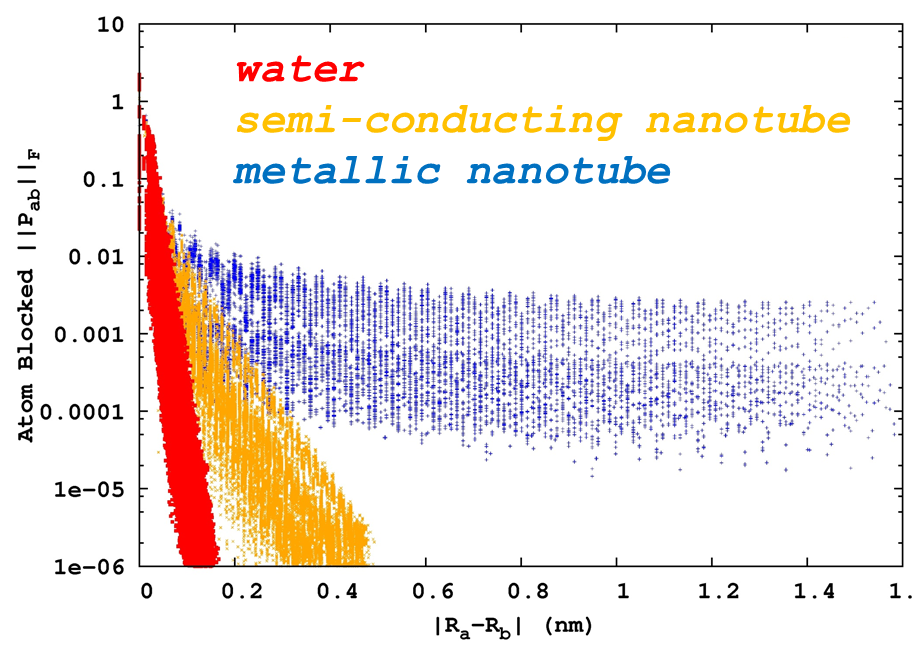
\includegraphics[width=3.5in]{decay_picture.png}
  \caption{Examples from electronic structure of decay for the
    spectral projector (gap shifted sign function) with respect to
    local (atomic) support.  Shown is decay for systems with
    correlations that are short (insulating water), medium
    (semi-conducting 4,3 nanotube), and long (metallic 3,3 nanotube)
    ranged, from exponential (insulating) to algebraic (metallic). }
\end{figure}

A well conditioned matrix $\mat{s}$ may often correspond to matrix
sign and inverse square root functions with rapid exponential decay,
and be amenable to {\em ad hoc} matrix truncation or ``sparsification'', 
$\bar{\mat{s}} = \mat{s}+ \mat{\epsilon}^{\mat{s}}_\tau$,
where $\mat{\epsilon}^{\mat{s}}_\tau$ is the error introduced
according to some criterion $\tau$.  
%Supporting this approximation are useful bounds to matrix function elements \cite{Benzi99b, }.
The criterion $\tau$ might be a drop-tolerance,
$\epsilon^{\mat{s}}_{\tau} = \{-s_{ij}*\hat{\mat{e}}_i \, | \, |s_{ij}|<\tau \}$,
a radial cutoff,
$\epsilon^{\mat{s}}_{\tau} = \{-s_{ij}*\hat{\mat{e}}_i \, | \, \lVert \mat{r}_i - \mat{r}_j \rVert > \tau \}$,
or some other approach to truncation, perhaps involving a sparsity
pattern chosen {\em a priori} for computational expedience.
Then, the sparse general matrix-matrix multiply ($\tt{SpGEMM}$)
\cite{Gustavson78, Toledo97, challacombe00, bowler00} may be employed, yielding fast
solutions for multiplication rich iterations with fill-in modulated by truncation.
%These and related incomplete/inexact approaches to the computation of
%sparse approximate matrix functions often lead to ${\cal O}(n)$
%algorithms, finding wide use in technologically important
%preconditioning schemes, the information sciences, electronic
%structure and many other disciplines. 
Comprehensive surveys of these
methods in the numerical linear algebra are given by Benzi
\cite{Benzi99,Benzi02}, and by Bowler \cite{Bowler12} and Benzi \cite{Benzi13}
for electronic structure.

Often however, matrix truncation is ineffective for ill-conditioned problems, 
because of slow decay, and because of increased numerical sensitivities to poorly 
controlled (absolute) truncation errors, {\em e.g.}~in the matrix-product:
\begin{equation} \label{sparseapprox}
\overline{ \mat{a} \cdot \mat{b} }\; = \; \mat{a}\cdot\mat{b} \; +\; \mat{\epsilon}^{\mat{a}}_\tau \cdot \mat{b} \;+\;
 \mat{a} \cdot \mat{\epsilon}^{\mat{b}}_\tau  \; + \;   {\mathcal O}(\tau^2) \, .
\end{equation}
An alternative approach is to find a reduced rank approximation closed under the operations of interest. 
However, compression to a reduced rank may be expensive if the rank is not much much smaller than the dimension.
Both of these methods, truncation and rank reduction, are focused on matrix data as the target for compression.
In this contribution, our target for compression is instead the matrix product itself.  For problems with
decay, we show that an underlying metric locality, together with a new form of algebraic locality, 
can lead to complexity reduction under contracting iteration and the $n$-body occlusion-cull. The organization of 
this paper follows.

\tableofcontents

\section{$\tt SpAMM$}
%\section{Sparse Approximate Matrix Multiplication ($\tt SpAMM$)}

In this contribution, we further develop the $\tt SpAMM$ $n$-body solver for the
approximation of matrix functions with decay, based on the quadtree data structure 
\cite{Wise:1984:RMQ:1089389.1089398,springerlink:10.1007/3-540-51084-2_9,
      Samet:1990:DAS:77589,Wise1990,Wise:Ahnentafel,
      Lorton:2006:ABL:1166133.1166134,Samet:2006:DBDS,Adams:2006:SOS,bader13},
\begin{equation}
\mat{a}^i = \begin{bmatrix} \,  \mat{a}^{i+1}_{00} \, & \,  \mat{a}^{i+1}_{01} \,  
\\[0.2cm]  \, \mat{a}^{i+1}_{10} \,  & \,\mat{a}^{i+1}_{11} \, \end{bmatrix} \, .
\end{equation}

For matrices with decay, orderings that preserve data-locality often 
lead to blocked-by-magnitude or other structures that concentrate data in 
well segregated neighborhoods; blocks, diagonals, bands \& {\em etc}.   
Then, matrix elements of like size may be efficiently resolved by the quadtree data structure 
\cite{Wise:1984:RMQ:1089389.1089398,springerlink:10.1007/3-540-51084-2_9,
      Samet:1990:DAS:77589,Wise1990,Wise:Ahnentafel,
      Lorton:2006:ABL:1166133.1166134,Samet:2006:DBDS,Adams:2006:SOS,Bock2013,bader13}.

Increasing data concentration allows to avoid white space in queries and 
computation, which is compressive for algorithms that can exploit these properties.
One common example of such data locality corresponds to an underlying order
of particles, elements, support functions \& {\em etc.} with a space filling curve 
\cite{Aluru:1997:SFC,Bader:2006:SFC,Campbell:2003:SFC,Devine:2005:SFC,Lashuk:2009:SFC, 
Gunther2006,Camata2010,1298805,Bock2013,bader13}

\subsection{Occlusion-cull }

The Sparse Approximate Matrix Multiply ($\tt SpAMM$) carries out occlusion-culling to find only the
most important sub-volumes in an approximate matrix product. 
$\tt SpAMM$ has evolved from a row-column oriented skipout mechanism within the
BCSR and DBCSR structures \cite{challacombe1999simplified,Challacombe:2000:SpMM}, 
to hierarchical approaches based on the quadtree and related to 
the occlusion-culling found in advanced mechanics and graphics methodologies \cite{Challacombe2010}, 
with occlusion the avoidance of unnecessary tree-work and culling the collection of significant tasks. 
We again amend the $\tt SpAMM$ occlusion-cull,  with the recursion
\begin{widetext}
\begin{equation}\label{newspamm}
\mat{a}^{i} \ot \mat{b}^{i} =
\left\{
        \begin{array}{ll}
                 \emptyset \quad \tt{if}\quad \lVert \mat{a}^i \rVert \lVert \mat{b}^i \rVert < \tau \lVert a \rVert \lVert b \rVert \\[0.2cm]
                 \mat{a} ^i \cdot \mat{b}^i \quad  \tt{if}(i=\tt{leaf}) \\[0.2cm]
\begin{bmatrix} \mat{a}^{i+1}_{00} \ot \mat{b}^{i+1}_{00} +\mat{a}^{i+1}_{01} \ot \mat{b}^{i+1}_{10} \; , \; &
                \mat{a}^{i+1}_{00} \ot \mat{b}^{i+1}_{01} +\mat{a}^{i+1}_{01} \ot \mat{b}^{i+1}_{11}  \\[0.2cm]
                \mat{a}^{i+1}_{00} \ot \mat{b}^{i+1}_{01} +\mat{a}^{i+1}_{01} \ot \mat{b}^{i+1}_{11} \; , \; &
                \mat{a}^{i+1}_{00} \ot \mat{b}^{i+1}_{01} +\mat{a}^{i+1}_{01} \ot \mat{b}^{i+1}_{11}
\end{bmatrix}  \quad \tt{else}
                \end{array}
              \right.  \, ,
\end{equation}
\end{widetext}
which bounds the relative occlusion error
\begin{equation}\label{bound}
\frac{\lVert \mat{\Delta}^{a \cdot b}_{\tau} \rVert}{n^2 }  \, \leq \, \tau \, \lVert \mat{a} \rVert  \,  \lVert \mat{b} \rVert \, ,
\end{equation}
that occurs in the approximate product
\begin{equation}
\widetilde{\mat{a}\cdot \mat{b}} \,  \equiv \, \mat{a} \ot \mat{b} \,
  = \, \mat{a} \cdot \mat{b} + \mat{\Delta}^{a \cdot b}_{\tau} \, ,
\end{equation}
where $\lVert \cdot \rVert \equiv \lVert \cdot \rVert_F$ is sub-multiplicative \cite{Kahan2013}.

\subsection{Bound}

We now prove (\ref{bound}).

\begin{prop}
\label{lem:SpAMM mult, prop}
Let $\tau_{A,B} = \tau \| A \| \| B \| $. Then for each $i,j$,

\[
\left|\left(A\otimes_{\tau}B\right)_{ij}-\left(A\cdot B\right)_{ij}\right|\leq n\tau_{A,B},
\]
and
\[
\left\Vert A\otimes_{\tau}B-A\cdot B\right\Vert _{F}\leq n^{2}\tau_{A,B}.
\]
\end{prop}

\begin{proof}


We first show the following technical result: it is possible to choose $\alpha_{lij}\in\left\{ 0,1\right\} $ such that 

\begin{equation}
\left(A\otimes_{\tau}B\right)_{ij}=\sum_{l=1}^{n}A_{il}B_{lj}\alpha_{lij},\label{eq:spamm form, lemma}
\end{equation}
In addition, if $\alpha_{lij}=0$, then \textup{$\left|A_{il}\right|\left|B_{lj}\right|<\tau_{A,B}$. }. To show this, we use 
induction on the number $k_{\max}$ of levels. 

First, if $k_{\max}=0$,
\[
A\otimes_{\tau}B=\begin{cases}
0 & \,\,\text{if}\,\,\left\Vert A\right\Vert _{F}\left\Vert B\right\Vert _{F}<\tau_{A,B},\\
A\cdot B & \,\,\text{else}.
\end{cases}
\]
Therefore, $A\otimes_{\tau}B$ is of the form (\ref{eq:spamm form, lemma})
with either all $\alpha_{lij}=0$ or all $\alpha_{lij}=1$. Moreover,
if $\alpha_{lij}=0$, then $\left|A_{il}\right|\left|B_{lj}\right|\leq\left\Vert A\right\Vert _{F}\left\Vert B\right\Vert _{F}<\tau_{A,B}$. 

Now assume that the claim holds for $k_{\max}-1$. We show that it
holds for $k_{\max}$. Indeed, if $\left\Vert A\right\Vert _{F}\left\Vert B\right\Vert _{F}<\tau_{A,B}$,
we have that $A\otimes_{\tau}B=0$, which is of the form (\ref{eq:spamm form, lemma})
with all $\alpha_{lij}=0$. Also, if $\alpha_{lij}=0$, then $\left|A_{il}\right|\left|B_{lj}\right|<\left\Vert A\right\Vert _{F}\left\Vert B\right\Vert _{F}<\tau_{A,B}$.

Now assume that $\left\Vert A\right\Vert _{F}\left\Vert B\right\Vert _{F}\geq\tau_{A,B}$.
Then
\[
A\otimes_{\tau}B=\left(\begin{array}{cc}
A_{11}\otimes_{\tau}B_{11}+A_{12}\otimes_{\tau}B_{21} & A_{11}\otimes_{\tau}B_{12}+A_{12}\otimes_{\tau}B_{22}\\
A_{21}\otimes_{\tau}B_{11}+A_{22}\otimes_{\tau}B_{21} & A_{21}\otimes_{\tau}B_{21}+A_{22}\otimes_{\tau}B_{22}
\end{array}\right).
\]
We need to consider four cases: $i\leq n/2$ and $j\leq n/2$, $i>n/2$
and $j>n/2$, $i>n/2$ and $j\leq n/2$, and, finally, $i>n/2$ and
$j>n/2$. Since the analysis is similar for all four cases, we only
consider $i\leq n/2$ and $j\leq n/2$. We have that 
\begin{eqnarray*}
\left(A\otimes_{\tau}B\right)_{ij} & = & \left(A_{11}\otimes_{\tau}B_{11}+A_{12}\otimes_{\tau}B_{21}\right)_{ij}\\
 & = & \sum_{l=1}^{n/2}\left(A_{11}\right)_{il}\left(B_{11}\right)_{lj}\alpha_{lij}^{(1)} + \\
 & & \,\,\,\,\,\,\,\, \sum_{l=1}^{n/2}\left(A_{12}\right)_{il}\left(B_{21}\right)_{lj}\alpha_{lij}^{(2)}\\
 & = & \sum_{l=1}^{n}A_{il}B_{lj}\alpha_{lij},
\end{eqnarray*}
where we used the induction hypothesis in the second equality.

Now suppose that $\alpha_{lij}=0$ for some $l$. Then $\tilde{\alpha}_{lij}^{(1)}=0$
if $l\leq n/2$ or $\tilde{\alpha}_{l-n/2,ij}^{(2)}=0$ $l>n/2$.
If, e.g., $\tilde{\alpha}_{l-n/2,ij}^{(2)}=0$, then $\left|A_{il}\right|\left|B_{lj}\right|=\left|\left(A_{12}\right)_{i,l-n/2}\right|\left|\left(B_{21}\right)_{l-n/2,j}\right|<\tau_{A,B}$,
where we used the induction hypothesis in the final inequality. The
analysis for $l\leq n/2$ is similar, and the claim
follows.

We can now finish the proof of Proposition~\ref{lem:SpAMM mult, prop}. Indeed, by (\ref{eq:spamm form, lemma}),
\begin{eqnarray*}
\left|\left(A\otimes_{\tau}B\right)_{ij}-\left(A\cdot B\right)_{ij}\right| & \leq & \sum_{l=1}^{n}\left|A_{il}B_{lj}\right|\left|\alpha_{lij}-1\right|\\
 & = & \sum_{\alpha_{lij}=0}\left|A_{il}B_{lj}\right|.
\end{eqnarray*}
In addition, if $\alpha_{lij}=0$, then $\left|A_{il}B_{lj}\right|<\tau_{A,B}$
and the lemma follows.

\end{proof}

\subsection{Related research}\label{relatedr} 

$\tt SpAMM$ is perhaps most closely related to the Strassen-like branch of fast matrix multiplication 
\cite{springerlink:10.1007/BF02165411,DDH07,Ballard2014,LeGall:2014:PTF:2608628.2608664,Ambainis15},
and also methods for group theoretical embedding allowing fast polynomial multiplication 
\cite{cohn2003group,cohn2005group,Umans:2006:GAM:1145768.1145772}.
In the Strassen-like approach, disjoint tensor volumes are omitted recursively, 
while in the $\tt SpAMM$ approach to fast multiplication, the numerically least significant 
tensor intermediates in the n\"{a}ive product space are omitted recursively, with error bounded by Eq.~(\ref{bound}).  
Also, these methods for fast matrix multiplication are {\bf \em stable} \cite{DDH07}.

$\tt SpAMM$ is a $n$-body method for fast matrix multiplication, related to the 
generalized methods popularized by Grey \cite{Gray01,Gray2003}. In our development,
generalization reflects the {\bf \em genericity} of recursive data access 
\cite{genericityindata,Geerts2002,Samet:2006:DBDS,Gottschling2009},
enabling new math supported by range queries, metric queries, higher dimensional queries and so on, but with common frameworks, 
structures, skeletons, run-times \& {\em etc.}  
So far, we have prototyped $n$-body solvers for the  mainstay problems in modern electronic structure theory, 
including the Fock exchange \cite{challacombe2014n}, 
semi-local exchange-correlation functionals \cite{Challacombe:2000:HiCu,10.1063/1.1568734}, 
the Hartree (Coulomb) interaction \cite{Challacombe:Review,Challacombe:1996:QCTCb,Challacombe:1997:QCTC,Challacombe:1997:PFMM}, 
matrix sign function \cite{Challacombe2010,BockCK14} 
and the matrix inverse square root (this work).
%This contribution is cornerstone for the simplification and evolution of these solvers.  

%Top-down $n$-body recursion and breadth-first map-reduction may be viewed as two sides of 
%the same problem \cite{Aluru}.  
Emergent data frameworks, functional programming languages and other technologies that support generic recursion and 
skeletonizations \cite{Sarje2010a,Gonzalez-Velez:2010:SAS:1890754.1890757,CPE:CPE3087,rodrigues2014triolet,March} 
may enable exploitation of increasingly cheap (decentralized) concurrence by scientific $n$-body solvers, 
and also lower barriers to entry, enhance reliability, sustainability \& {\em etc.}
For centralized, distributed architectures, $n$-body methods offer well established protocols for turning spatial and metric locality into 
data and temporal locality \cite{Warren:1993:PHO:169627.169640,Warren:1995:HOT,Warren1995266,WarrenGordonBell1997,Warren2013}.  
Recently for example, Driscoll {\em et. al} showed perfect strong scaling and communication optimally 
for pairwise $n$-body methods \cite{Driscoll2013}.   Bridging the gap between 
$n$-body solver and fast matrix multiplication, we recently demonstrated strong scaling for fast matrix multiplication 
($\tt SpAMM$) \cite{BockCK14}.  

This work offers a data local alternative to fast non-deterministic methods for sampling the product, 
which include sketching \cite{Sarlos2006,Drineas2006,Mahoney2012,Pagh2013,Woodruff2015},
joining \cite{Mishra92,Hoel94,Jacox03,Chen07,Amossen09,Lieberman08,Kim09}, 
sensing \cite{iwen2009note} and probing \cite{chiu2012matrix}.  These  methods may involve probabilistic 
and on the fly sampling, with the potential for complexity reduction in the case of random distributions or related assumptions. 
$\tt SpAMM$  also employs on the fly weighted sampling,  but with 
compression through locality, brought about by algebraic correlations (towards identity) and also through structured metric localities.

% Methods that achieve compression in the stream of product intermediates are different from reduced rank algorithms that achieve 
% matrix compression in a step that preceeds multiplication (seperability)  \cite{}.   However, matrix compressions are 
% generally compatible with the quadtree, as are additional fast (generalized) solvers that add complex functionality ({\em e.g.} 
% in electronic structure theory \cite{}).  Thus, generality 
% and interoperability may enable deeply layered, thin and generic solvers easy access to in place data. 
% Further, language support may provide simple (skeletonized) frameworks for generic recursion, 
% offering opportunities to greatly simplify codebase at the systems level, 
% lowering barriers to entry and enhancing concurence (in the Erlang sense). 


Finally, this work is inspired broadly by Higham's work, particularly the 2005 paper by 
Higham, Mackey, Mackey and Tisseur \cite{higham2005} on square root iteration and the group structure of matrix functions.
Also, it is influenced by Chen and Chow's \cite{chen2014} approach to scaled NS iteration for ill-conditioned problems, and by 
the Helgaker group's work on NS iteration, whose notation we follow in part \cite{Jansik2007}.  

% which leads to a non-associative algebra and error flows with
% properties of the Lie bracket
% \begin{equation} \label{braket}
% \widetilde{\left[ \mat{a} , \mat{b} \right]} \equiv \mat{a} \ot \mat{b}-\mat{b} \ot \mat{a}
% =  \left[ \mat{a} , \mat{b} \right]
% + \ma\Delta}^{a\cdot b}_{\tau} -\mat{\Delta}^{b\cdot a}_{\tau} \,.
% \end{equation}

% Finally, the

\section{First Order Newton-Shulz Iteration}

There are two common, first order NS iterations; the sign iteration
and the square root iteration, related by the square, $\mat{I}\left(
\cdot \right)= {\rm sign}^2\left( \cdot \right) $.  These equivalent
iterations converge linearly at first, then enter a basin of stability
marked by super-linear convergence.  

\subsection{Sign iteration}

For the NS sign iteration, this basin is marked by a behavioral change
in the difference $\delta \mat{X}_k = \widetilde{\mat{X}}_k -\mat{X}_k
= {\rm sign} \left(\mat{X}_{k-1}+\delta \mat{X}_{k-1} \right) -{\rm
  sign} \left(\mat{X}_{k-1} \right)$, where $\delta \mat{X}_{k-1}$ is
some previous error.  The change in behavior is associated with the
onset of idempotence and the bounded eigenvalues of ${\rm sign}'\left(
\cdot \right)$, leading to stable iteration when ${\rm sign}'\left(
\mat{X}_{k-1} \right) \delta \mat{X}_{k-1} < 1 $.  Global perturbative
bounds on this iteration have been derived by Bai and Demmel
\cite{Bai98usingthe}, while Byers, He and Mehrmann \cite{} developed
asymptotic bounds.  The automatic stability of sign iteration is a
well developed theme in Ref.\cite{Higham08}.

\subsection{Square root iteration}
In this work, we are concerned with resolution of the identity
\begin{equation}
\mat{I} \left( \mat{s} \right) =\mat{s}^{1/2} \cdot \mat{s}^{-1/2} \, ,
\end{equation}
and its low-complexity computation with fast methods.  

Starting with eigenvalues rescaled to the domain $(0,1]$ with the easily obtained 
largest eigenvalue,   $\mat{s} \leftarrow \mat{s}/s_{N-1}$, and with $\mat{z}_0=\mat{I}$ and 
$\mat{x}_0=\mat{y}_0=\mat{s}$, the corresponding canonical,  ``dual'' channel square root iteration is:
\begin{eqnarray}\label{cannonical}
\mat{y}_k &\leftarrow& h_\alpha \left[ \mat{y}_{k-1} \cdot \mat{z}_{k-1} \right] \cdot \mat{y}_{k-1}  \nonumber \\
\mat{z}_k &\leftarrow& \mat{z}_{k-1} \cdot h_\alpha \left[ \mat{y}_{k-1} \cdot \mat{z}_{k-1} \right] \; ,
\end{eqnarray}
converging as ${\mat{y}}_k \rightarrow \mat{s}^{1/2}$, ${\mat{z}}_k \rightarrow \mat{s}^{-1/2}$ and
${\mat{x}}_k \rightarrow {\mat{I}}$, with eigenvalues aggregated towards 1 by 
the NS map $h_\alpha[\mat{x}]=\frac{\sqrt{\alpha}}{2} \left(3-\alpha \mat{x} \right)$ \cite{Higham08,higham2005}.  
As in the case of sign iteration, this canonical iteration was shown by Higham, Mackey, Mackey and
Tisseur \cite{higham2005} to remain strongly bounded in the super-linear regime, by idempotent Frechet derivatives about the fixed point
$\left(\mat{s}^{1/2},\mat{s}^{-1/2}\right)$, in the direction $\left(
\delta \mat{y}_{k-1} , \delta \mat{z}_{k-1} \right)$:
\begin{eqnarray}
\delta \mat{y}_k &=& \frac{1}{2} \delta \mat{y}_{k-1} - \frac{1}{2} \mat{s}^{1/2} \cdot \delta \mat{z}_{k-1} \cdot \mat{s}^{1/2} \\
\delta \mat{z}_k &=& \frac{1}{2} \delta \mat{z}_{k-1} - \frac{1}{2} \mat{s}^{-1/2} \cdot \delta \mat{y}_{k-1} \cdot \mat{s}^{-1/2} \;.
\end{eqnarray}
In addition to the dual channel instance, we also consider the ``single'' channel version of square root iteration,
\begin{eqnarray}\label{single}
\mat{z}_k &\leftarrow& \mat{z}_{k-1} \cdot h_\alpha \left[ \mat{x}_{k-1} \right] \; , \nonumber \\
\mat{x}_k &\leftarrow&  \mat{z}^\dagger_{k} \cdot \mat{s} \cdot \mat{z}_{k} \; .
\end{eqnarray}

\subsection{Mapping}\label{map}
The NS logistic map for the square root iteration is $h_\alpha[\mat{x}]=\frac{\sqrt{\alpha}}{2} \left(3-\alpha \mat{x} \right)$, 
with the initial rate of convergence controlled by $h'_\alpha$ and the smallest eigenvalue, $x_0$. 
various schemes for controlling the values $\alpha$ towards convergence, 
notably  by Pan and Schreiber \cite{Pan1991}, and more recently, Jie and Chen \cite{chen2014}, who demonstrated  $\tt 2 \times$
acceleration for very ill-conditioned problems with their new scaling approach. 

In addition to scaling of the NS logistic, we introduce a stabilizing map that accounts for eigenvalues 
tossed out of bounds by $\ot$. This stabilization is the transformation $[0,1] \rightarrow [0+\varepsilon, 1-\varepsilon]$
(shift and scale), carried out prior to application of the logistic.   

The most important aspect of these scaling and stabilization maps is to turn them off towards convergence.  Conventional methods 
often compute a lowest eigenvalue to monitor convergence \cite{Pan1991,chen2014}, but this may be too expensive for ill-conditioned problems. 
Alternatively, we monitor convergence simply with the relative trace error, 
$t_k = \left( n - {\rm tr} \, \widetilde{\mat{x}}_k \right) n^{-1}$.  
Then, empirically developed sigmoidal functions are used to damp the scaling parameter to unity, 
\begin{equation}
\alpha(t) = {\tt 1.} + {\tt 1.85}  \times \left( 1+e^{-{\tt 50.}(t-{\tt .35})}  \right)^{-1} 
\end{equation}
and the stability parameter to zero, 
\begin{equation}
\varepsilon(t) = {\tt .1} \times \left( 1+e^{-{\tt 75.}(t-{\tt .30})}  \right)^{-1} \, .
\end{equation}
These functions are used throughout. 

\section{Error Flows in Square Root Iteration}

\subsection{Stability}

% There are a number of equivalent instances of the square root iteration, related by commutations and transpositions. 
% Nominally, $\mat{y}^{\rm dual}$ is equivalent to $\mat{y}^{\rm single}_k \equiv \mat{z}^\dagger_{k} \cdot \mat{s}$.  
% However, with ill-conditioning and in only double precision, these two instances may diverge rapidly due to compounding  errors.
% In the case of the dual iteration, the $\widetilde{\mat{y}}^{\rm dual}_k$ channel does not retain contact with the eigenvectors of $\mat{s}$, 
% and can diverge easily from this basis. In the single instance, conection with $\mat{s}$ is retained at each step, but at the price 
% the update involving a broad spectral resolution, {\em e.g.} involving $\mat{s}^{-1/2} \cdot \mat{s}$  at convergence. 

Stability in the square root iteration is determined  by the differential 
\begin{equation} \label{firstorderdual}
\delta \mat{x}_k = \,  { \mat{x}}_{\delta \widehat{\mat{y}}_{k-1}}  \, {\scriptstyle \times} \, \delta y_{k-1}
                 \, + \,  { \mat{x}}_{\delta \widehat{\mat{z}}_{k-1}}  \, {\scriptstyle \times} \, \delta z_{k-1}  \, + {\cal O}(\tau^2) 
\end{equation}
which must remain bounded below one to avoid divergence.   The corresponding Fr\"{e}chet derivatives are
\begin{equation}
  \mat{x}_{\delta \widehat{ \mat{y}}_{k-1}}
= \lim_{\tau \rightarrow 0} \slantfrac{ \mat{x} \left( \mat{y}_{k-1} + \tau \delta \widehat{\mat{y}}_{k-1} ,  {\mat{z}}_{k-1}  \right)
                                     -\mat{x}_k    }{\tau} 
 \end{equation}
and
 \begin{equation}
 \mat{x}_{\delta \widehat{ \mat{z}}_{k-1}} = \lim_{\tau \rightarrow 0}
\slantfrac{ \mat{x} \left( {\mat{y}}_{k-1} , \mat{z}_{k-1} +\tau  \delta \widehat{\mat{z}}_{k-1} \right) - \mat{x}_k   }{\tau}  \, , 
 \end{equation}
along unit directions of the previous errors $\delta \widehat{\mat{y}}_{k-1}$ and $\delta \widehat{\mat{z}}_{k-1}$, by an amount
determined by the displacements $\delta y_{k-1} = \lVert \delta \mat{y}_{k-1} \rVert$  and  $\delta z_{k-1}=\lVert \delta \mat{z}_{k-1} \rVert$.
In the single instance, we have simply:
\begin{equation} \label{firstordersingle}
\delta \mat{x}_k = \,  { \mat{x}}_{\delta \widehat{\mat{z}}_{k-1}}  \, {\scriptstyle \times} \, \delta z_{k-1}  \, + {\cal O}(\tau^2)  \, .
\end{equation}

This formulation makes plain changes about the resolvent, separating orientational effects 
of the directional derivatives, set mostly by the underlying exact linear algebra, from 
changes to error displacements, which involve both the action of derivatives on previous errors,  as well as 
current $\tt SpAMM$ occlusion errors.

\subsection{Fr\"{e}chet derivatives}
%\subsubsection{Dual}
 
In the dual instance, Fr\"{e}chet derivatives occurring in Eq.~(\ref{firstorderdual}) are:

% \begin{equation}
%   \mat{x}_{\delta \widehat{ \mat{y}}_{k-1}}
% =   \mat{y}_{\delta \widehat{ \mat{y}}_{k-1}} \cdot \mat{z}_{k}  + \mat{y}_{k}  \cdot \mat{z}_{\delta \widehat{ \mat{y}}_{k-1}}
%  \end{equation}
% and
%  \begin{equation}
%  \mat{x}_{\delta \widehat{ \mat{z}}_{k-1}} =
% \mat{y}_{\delta \widehat{ \mat{z}}_{k-1}} \cdot \mat{z}_{k}  + \mat{y}_{k}  \cdot \mat{z}_{\delta \widehat{ \mat{z}}_{k-1}} \, .
%  \end{equation}


% For $\mat{x}_{\delta \widehat{ \mat{y}}_{k-1}}$ we have
% \begin{multline}
%  \mat{y}_{\delta \widehat{ \mat{y}}_{k-1}} = h_\alpha \left[ \mat{x}_{k-1} \right] \cdot \delta \widehat{\mat{y}}_{k-1} \\
%                                      + h'_\alpha \cdot \delta \widehat{\mat{y}}_{k-1} \cdot \mat{z}_{k-1} \cdot \mat{y}_{k-1}
% \end{multline}
% and
% \begin{equation}
%  \mat{z}_{\delta \widehat{ \mat{y}}_{k-1}} =  \mat{z}_{k-1} \cdot h'_\alpha \delta \widehat{\mat{y}}_{k-1} \cdot \mat{z}_{k-1}
% \end{equation}
% yeilding
% Also, for $\mat{x}_{\delta \widehat{ \mat{z}}_{k-1}}$ we have
% \begin{equation}
%  \mat{y}_{\delta \widehat{ \mat{z}}_{k-1}} =  {\mat{y}}_{k-1} \cdot  h'_\alpha \delta \widehat{ \mat{z}}_{k-1} \cdot  \mat{y}_{k-1}
% \end{equation}
% and
% \begin{multline}
%  \mat{z}_{\delta \widehat{ \mat{z}}_{k-1}} = \delta \widehat{\mat{z}}_{k-1} \cdot   h_\alpha \left[ \mat{x}_{k-1} \right] \\
%                                      + \mat{z}_{k-1} \cdot {\mat{y}}_{k-1} \cdot h'_\alpha \delta \widehat{\mat{z}}_{k-1}  \; ,
% \end{multline}
% yeilding

\begin{multline}\label{dxdy}
 \mat{x}_{\delta \widehat{ \mat{z}}_{k-1}} =  {\mat{y}}_{k-1} \cdot  h'_\alpha \delta \widehat{ \mat{z}}_{k-1} \cdot  \mat{y}_{k-1}  \cdot \mat{z}_{k} \\
\qquad + \mat{y}_k \cdot  \delta \widehat{\mat{z}}_{k-1} \cdot   h_\alpha \left[ \mat{x}_{k-1} \right] \\
\qquad \qquad +  \mat{y}_{k} \cdot  \mat{z}_{k-1} \cdot {\mat{y}}_{k-1} \cdot h'_\alpha \delta \widehat{\mat{z}}_{k-1} \, ,
\end{multline}
and 
\begin{multline}\label{dxdz}
  \mat{x}_{\delta \widehat{ \mat{y}}_{k-1}} = h_\alpha \left[ \mat{x}_{k-1} \right]  \cdot \delta \widehat{\mat{y}}_{k-1} \cdot \mat{z}_{k} \\
+  h'_\alpha  \delta \widehat{\mat{y}}_{k-1} \cdot \mat{z}_{k-1} \cdot  \mat{y}_{k-1} \cdot  \mat{z}_{k} \\
 + \mat{y}_{k} \cdot \mat{z}_{k-1} \cdot h'_\alpha \delta \widehat{\mat{y}}_{k-1} \cdot \mat{z}_{k-1}  \, .
\end{multline}


Closer to the fixed point orbit,  $\mat{y}_k \cdot \mat{z}_{k-1} \rightarrow \mat{I}$, $\mat{y}_{k-1} \cdot \mat{z}_{k} \rightarrow \mat{I}$,
$h_\alpha \left[ \mat{x}_{k} \right] \rightarrow \mat{I}$ and $h'_\alpha \rightarrow - \frac{1}{2}$ \cite{higham2005}.  Then,

\begin{equation} \label{yorbit}
 \mat{x}_{\delta \widehat{ \mat{y}}_{k-1}} \rightarrow \delta \widehat{\mat{y}}_{k-1} \cdot \left( \mat{z}_k-\mat{z}_{k-1} \right)
\end{equation}
and
\begin{equation} \label{zorbit}
 \mat{x}_{\delta \widehat{ \mat{z}}_{k-1}} \rightarrow \left( \mat{y}_k-\mat{y}_{k-1} \right) \cdot \delta \widehat{\mat{z}}_{k-1} .
\end{equation}
Likewise, in the single channel instance:
\begin{multline}
 \mat{x}_{\widehat{\mat{z}}_{k-1}} \rightarrow  \left(  \mat{z}_{k} - \mat{z}_{k-1} \right)^\dagger \cdot \mat{s} \cdot \delta \widehat{\mat{z}}_{k-1} \\
+  \, \delta \widehat{\mat{z}}^\dagger_{k-1} \cdot  \mat{s}  \cdot \left(  \mat{z}_{k} - \mat{z}_{k-1} \right)  \, .
\end{multline}

About the fixed point then, error flow in the $\mat{y}_k$ and the $\mat{z}_k$ channels is tightly quenched,
corresponding to $\mat{x}_{\delta \widehat{\mat{x}}_{k-1}} \rightarrow  \mat{I}$  and identity iteration \cite{higham2005}.

\subsection{Displacements}
Countering orientational convergence,  determined almost entirely by the underlying exact iterations, is the 
the compounding displacement error, determined by $\tt SpAMM$ occlusion in each of three products, at each step, and also
involving previous errors.  Here, we look at just the displacement $\delta \mat{z}_{k-1}$,
which has the largest potential for divergence as we argue here and show numerically in the following section. 

Including the $\tt SpAMM$ error in the $\widetilde{\mat{z}}_{k-1}$ update we have:
\begin{eqnarray} \label{widetildez}
 \widetilde{\mat{z}}_{k-1} &=&  \widetilde{\mat{z}}_{k-2}  \, \ot \, h_\alpha[\widetilde{\mat{x}}_{k-2}]\\ \nonumber
&=& \Delta^{\widetilde{\mat{z}}_{k-2} \cdot h_\alpha \left[ \widetilde{\mat{x}}_{k-2}\right]}_\tau
+ \widetilde{\mat{z}}_{k-2} \cdot h_\alpha\left[ \widetilde{\mat{x}}_{k-2}\right] \, .
%\end{equation}
\end{eqnarray}
Then, with $ h_\alpha \left[ \widetilde{\mat{x}}_{k-2} \right]
=  h_\alpha \left[ \mat{x}_{k-2} \right] +  h'_\alpha  \delta \mat{x}_{k-2}$, and taking $\mat{z}_{k-1}$ from both sides, we find  
%Eq.~(\ref{widetildez}) yeilds 
\begin{multline}
 \delta {\mat{z}}_{k-1} =\Delta^{\widetilde{\mat{z}}_{k-2} \cdot h_\alpha \left[ \widetilde{\mat{x}}_{k-2}\right]}_\tau
\\ +\delta \mat{z}_{k-2} \cdot h_\alpha \left[\widetilde{\mat{x}}_{k-2} \right]
+ \mat{z}_{k-2} \cdot h'_\alpha \delta \mat{x}_{k-2}  \, ,
\end{multline}
which is bounded by 
% \begin{multline}
%  \delta {z}_{k-1} <
% \lVert \mat{z}_{k-2} \rVert \left( \;  \tau \, \lVert h_\alpha \left[\widetilde{\mat{x}}_{k-2} \right]  \rVert
% + h'_\alpha \delta {x}_{k-2} \right)  \\ +
% \delta {z}_{k-2}  \lVert h_\alpha \left[\widetilde{\mat{x}}_{k-2}  \right] \rVert 
% \end{multline}
 \begin{multline}\label{zdispalcementbound}
  \delta {z}_{k-1} <
 \lVert \mat{z}_{k-2} \rVert \left( \tau  \, \sigma_n  \, \lVert h_\alpha \left[\widetilde{\mat{x}}_{k-2} \right]  \rVert
 + h'_\alpha  \delta y_{k-2} \lVert z_{k-2} \rVert \right)  \\ 
 + \delta {z}_{k-2} \left( \lVert h_\alpha \left[\widetilde{\mat{x}}_{k-2}  \right] \rVert  + \lVert y_{k-2} \rVert \right) .
 \end{multline}

In Eq.~(\ref{zdispalcementbound}),  the term $h'_\alpha  \delta y_{k-2} { \lVert \mat{z}_{k-2} \rVert }^2$ is volatile, tending towards
$\delta y_{k-2} \, \kappa(\mat{s})/2$.  Because of this sensitivity, and because the $\mat{y}_k$ product channel maintains fidelity 
of the starting eigen-basis, we single out this ``sensitive'' product for a higher level of precision; $\tau_s \ll \tau$.
Still, we expect different behavior from the single instance $\widetilde{\mat{y}}_{k-1} = \widetilde{\mat{z}}^{\dagger}_{k-1} \, \ots \, \mat{s}$,
and the dual instance $\widetilde{\mat{y}}_{k-1} =  h_\alpha [\widetilde{\mat{x}}_{k-1}]  \ots \widetilde{\mat{y}}_{k-1} $.
This is because the spectral product is broader (resolving larger and smaller numbers) 
in the single instance and narrower in the dual instance.

\subsection{Most approximate but still stable}

\begin{figure}[h]
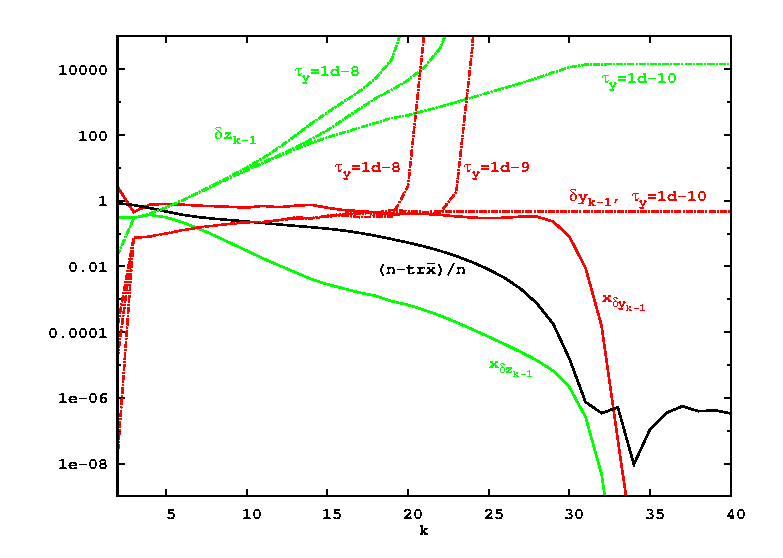
\includegraphics[width=3.5in]{fig_33_tube_cond_10_noscaling_33_nanotube_cond10_noscale_dual.eps}
%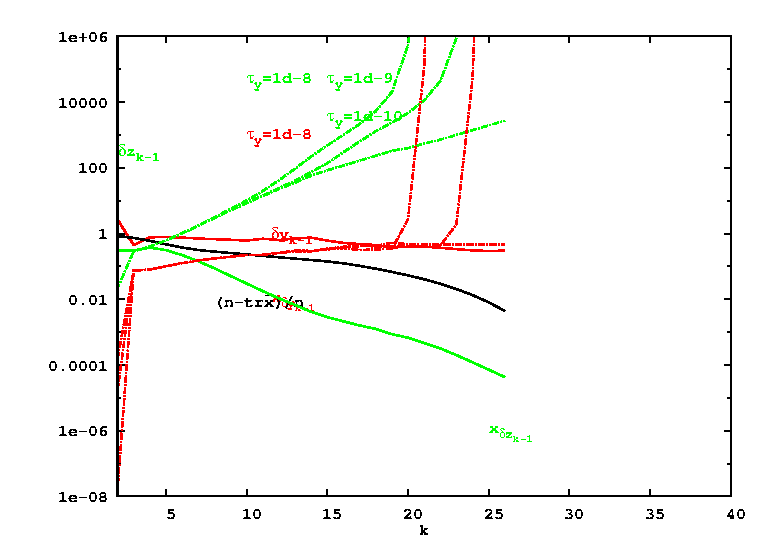
\includegraphics[width=3.5in]{fig_33_tube_cond_10_noscaling/33_nanotube_cond10_noscale_dual.eps}
\caption{Derivatives, displacements and trace error of the unscaled dual iteration.
Derivatives are full lines, whilst the displacements corresponding to $\tau_s=\{10^{-8}, 10^{-9}, 10^{-10}\}$
are the dashed lines.  The trace error is shown as a full black line. } \label{flow_noscale_dual}
\end{figure}

\begin{figure}[h] 
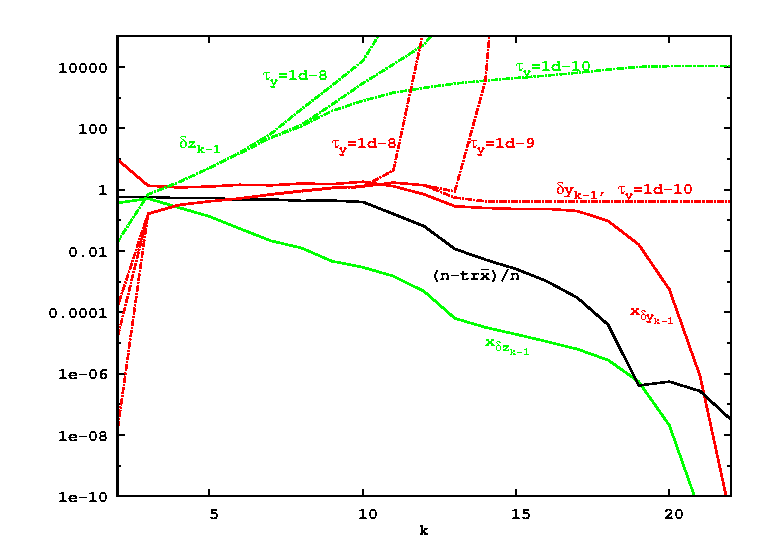
\includegraphics[width=3.5in]{fig_33_tube_cond_10_scaled_33_tube_k10_scale_dual.eps}
%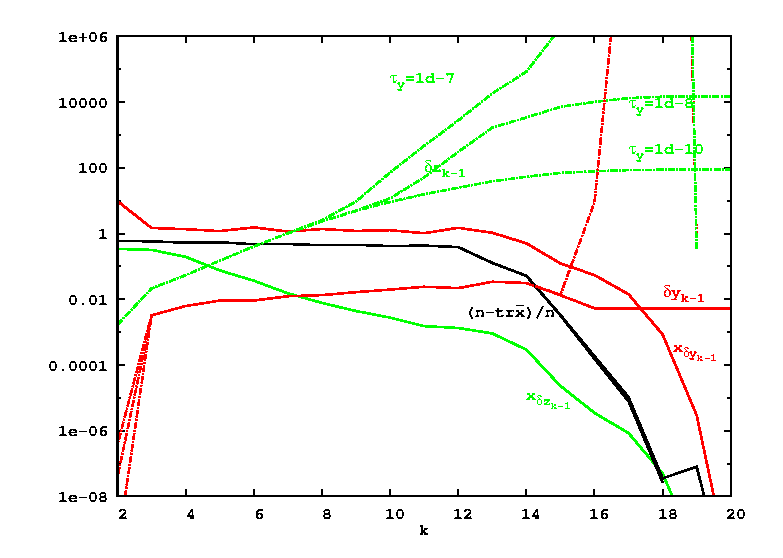
\includegraphics[width=3.5in]{fig_33_tube_cond_10_scaled/33_tube_k10_scale_dual.eps}
\caption{Derivatives, displacements and the approximate trace of the scaled dual iteration.
Derivatives are full lines, whilst the displacements corresponding to $\tau_s=\{10^{-8}, 10^{-9}, 10^{-10}\}$
are the dashed lines.  The trace error is shown as a full black line. }\label{flow_scaled_dual}
\end{figure}

\begin{figure}[h]
%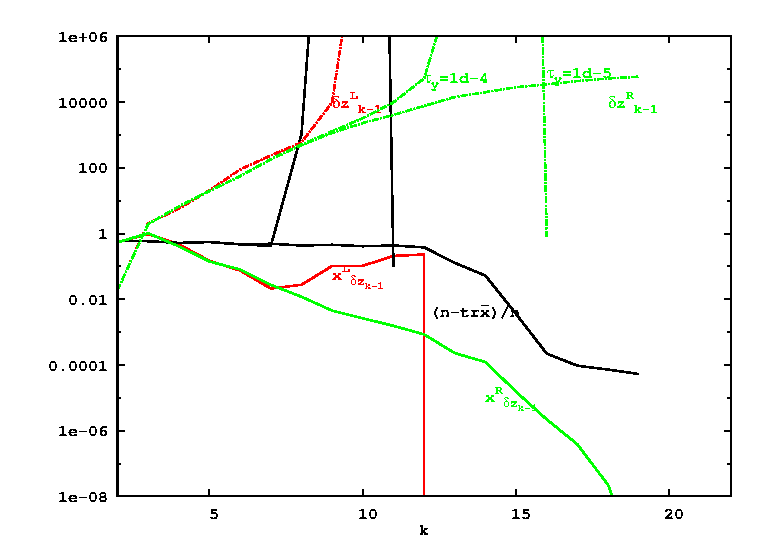
\includegraphics[width=3.5in]{fig_33_tube_cond_10_scaled/33_tube_k10_scale_stab.eps}
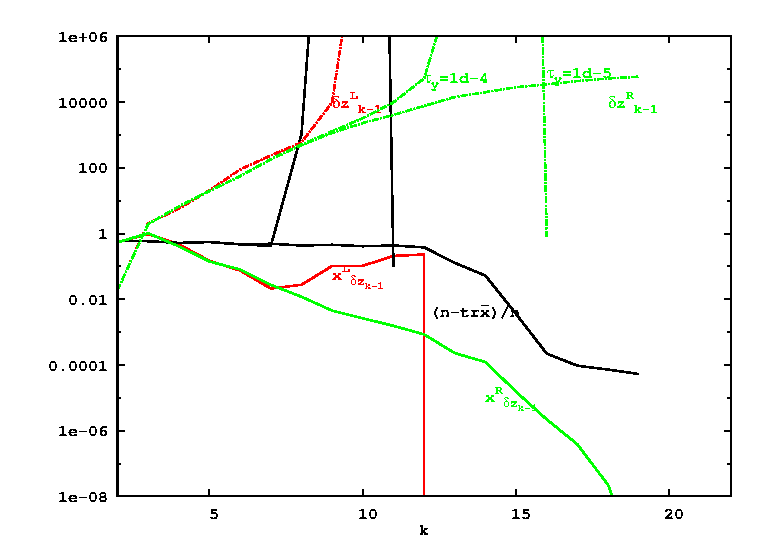
\includegraphics[width=3.5in]{fig_33_tube_cond_10_scaled_33_tube_k10_scale_stab.eps}
\caption{Derivatives, displacements and the approximate trace of the scaled single iteration.
Derivatives are full lines, whilst the displacements corresponding to $\tau_s=\{10^{-3}, 10^{-4}, 10^{-5}\}$
are the dashed lines.  The trace error is shown as a full black line. }\label{flow_scaled_stab}
\end{figure}

Experiments were carried out on the ill-conditioned $(\kappa(\mat{s})=10^{10})$ nanotube metric-matrices described in Appendix~\ref{data}.
We picked  $\tau ={\tt .001}$ and block size $b = 64$.  Then, we looked at stability with respect to the tighter $\tau_s$ threshold, 
the directional derivatives and the trace error.   

In Fig.~\ref{flow_noscale_dual}, unscaled results for the dual instance are shown.  In Fig.~\ref{flow_scaled_dual}, scaled results for the
dual instance are given, reclaiming approximately $2/3$ of the available $2 \times$ acceleration, with a $1/3$ penalty due to the
stabilization map described in Section \ref{map}. Then, in Fig.~\ref{flow_scaled_stab} we show results for the scaled single instance. 

Not shown is complete fill-in at convergence for even the most-approximate-yet-still-stable (MAYSS) value of $\tau_s$.  
Also, with a less forgiving stability map, we find interesting 
left/right differences;  namely, the right first product 
\begin{equation} 
\widetilde{\mat{x}}^R_k \leftarrow \widetilde{\mat{z}}^\dagger_{k} \, \ot  \, \left( \mat{s} \,  \ots \, \widetilde{\mat{z}}_{k-1}  \right) \; ,
\end{equation}
is  different from the left first product 
\begin{equation} 
\widetilde{\mat{x}}^L_k \leftarrow \left(  \widetilde{\mat{z}}^\dagger_{k} \, \ots \, \mat{s} \right) \,  \ot  \, \widetilde{\mat{z}}_{k-1} \; ,
\end{equation}
which is unsurprising.  All results shown correspond to the right-first protocol.

The stability map parameters discussed Section \ref{map} 
are tuned away from such sensitivities, and their local variation has a negligible impact on stability.  
Also not shown, the intermediate volumes (before fill in) behave very differently with scaling; in all cases, the product volumes,
proportional to the computational cost, are significantly increased by scaling.  In the remainder of this work, we won't look at scaling again.

\section{Regularization}\label{regularization}

Even for the most approximate but stable (MAYSS) approximations, our nanotube calculations become dense in both the data and task domains, 
even for very large $128 \times$ U.C. systems.  For these ill-conditioned iterations, broad spectral resolutions that involve products of 
large and small numbers correspond to delocalized products that are not tightly bound by the $\tt SpAMM$ approximation.   However, as 
we show later in Fig.~\ref{Lensing4}, similarly ill-conditioned problems may achieve substantial compression with just the MAYSS 
approximation. 

A systematic way to reduce ill-conditioning is through Tikhonov regularization \cite{neumaier1998solving,sarra2014}.
Regularization involves a small level shift of the eigenvalues,  $\mat{s}_\mu \leftarrow \mat{s}+\mu \mat{I}$, altering the 
condition number of the shifted matrix to  $\kappa( \mat{s}_\mu) = \frac{\sqrt{s^2_{n-1} + \mu^2}}{\sqrt{s^2_0+\mu^2}}$ \cite{sarra2014}.
%Regularization has an history in quantum chemistry \cite{}, image processing \cite{} and linear algebra \cite{}.   

Achieving substantial acceleration with severe ill-conditioning  may require a large level shift however, 
producing inverse factors of little practical use.  One approach to recover a more accurate inverse
factor is Riley's method based on Taylor's series \cite{sarra2014}; 
\begin{equation}
\mat{s}^{-1/2} = \mat{s}^{-1/2}_{\mu} \cdot \left( \mat{I}+\frac{\mu}{2} \mat{s}^{-1}_{\mu}
                                                   +\frac{3 \mu^2}{8} \mat{s}^{-2}_{\mu} + \dots
   \right) \; .
\end{equation}
For severely ill-conditioned problems and large level shifts, this expansion may converge very slowly. 
Also, adding powers of the full inverse may not be computationally effective. 

\subsection{Product representation}

We introduce an alternative representation of the regularized inverse factor;
\begin{equation} \label{spammsandwich}
\mat{s}^{-1/2} \equiv \bigotimes_{\substack{\tau=\tau_0 \\ \mu=\mu_0   } } {\left|\, \tau\, \mu \, ; \, \scriptstyle{\mat{s}^{-1/2}}  \right>}  \, ,
\end{equation}
which is a telescoping product of preconditioned ``slices'' 
starting with a most-approximate-yet-still-effective-by-one-order (MAYEBOO) preconditioner, 
$\mat{s}^{-1/2}_{\tau_0 \mu_0} \equiv {\left|\, \tau_0\, \mu_0 \, ; \, \scriptstyle{\mat{s}^{-1/2}}\right>}$\footnote{Braket notation marks 
the potential for asymmetries in the intermediate representation.}.  
This sandwich of generic, thinly sliced {\tt SpAMM} products allows to construct a nested scoping on precision via $\tau$, and in the 
effective condition number controlled by $\mu$.


% This scheme rests on three factors: ({\bf 1}) the ability to find a most agressive but still effective first slice,   
% corrective by one order in the condition, $\mu_0 = {\tt .1}$, and by one order in the precision, $\tau_0 ={\tt .1}$ (MAYEBOO), 
% ({\bf 2}) an optimal $\tau \, \mu$ scoping in Eq.~(\ref{spammsandwich})  and ({\bf 3}) optimized 
% maps for generic thin slices.  In the following, we demonstrate a first MAYEBOO preconditioner for the ill-conditioned 
% nano-tube problem, and then we sketch a naive approach to building the full inverse factor. 


\subsection{Effective by one order}

We look again at the $\kappa(\mat{s})=10^{10}$ nanotube series described in Appendix \ref{data},
this time with extreme regularization, $\mu_0={\tt .1}$, and at a finer granularity, $b=8$.
Culled $\mat{y}_k$ and $\mat{z}_k$ volumes (as percentage of the total work) for $36 - 128 \, \times$ the (3,3) unit cell
are shown for the MAYEBOO approximation in Fig.~\ref{regularized_stab} for the single instance, 
and in Fig.~\ref{regularized_dual} for the dual instance. 

The behavior of these implementations  is very different; in the single 
instance, a stable  iteration could not be found at precision $\tau_0=\tt .1$.  Stability could 
only be found at ${\tt .01}$, and that with a poorly contained trace error and cull-volumes 
that continue to inflate past convergence, with a conspicuous $\sqrt{k}$-like dependence.  
On the other hand, dual iteration volumes demonstrate
collapsing volumes and fast trapping of the trace error with resolution of the approximate identity.
%$\widetilde{\mat{I}}_{\tau_0\mu_0}$.  

We interpret these results as follows: The single instance sufferes from an increasingly broad resolution of spectral powers,
$\widetilde{\mat{y}}_k \rightarrow  \mat{s}^{-1/2}_{\tau_0 \mu_0} \oto \mat{s}_{\mu_0}$, which is  poorly bound by Eq.~(\ref{bound}). 
In the dual instance however, $\widetilde{\mat{y}}_k\rightarrow  \mat{I}_{\tau_0 \mu_0} \oto \mat{s}^{1/2}_{\tau_0 \mu_0}$
and $\widetilde{\mat{z}}_k \rightarrow  \mat{s}^{-1/2}_{\tau_0 \mu_0} \oto \mat{I}_{\tau_0 \mu_0}$, 
with Eq.~(\ref{bound}) tightening to
\begin{equation}\label{boundY}
\Delta^{\mat{I}_{\tau_0 \mu_0} \cdot \mat{s}^{1/2}_{\tau_0 \mu_0}} <  \tau n \lVert \mat{s}^{1/2}_{\tau_0 \mu_0} \rVert
\end{equation}
and 
\begin{equation}\label{boundZ}
\Delta^{ \mat{s}^{-1/2}_{\tau_0 \mu_0}\cdot \mat{I}_{\tau_0 \mu_0}}  <  \tau n \lVert \mat{s}^{-1/2}_{\tau_0 \mu_0} \rVert \, .
\end{equation}
This contraction to the plane diagonal is compressive, leading to computational complexities that should approach quadtree copy in place.   

\begin{figure}[h]
% 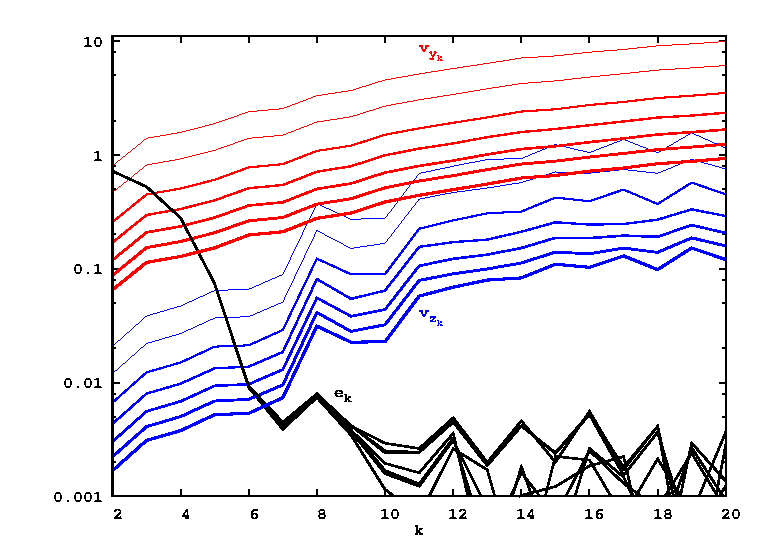
\includegraphics[width=3.5in]{fig_33_tube_cond_10_regularized/33_tube_k10_regularized_stab.eps}
 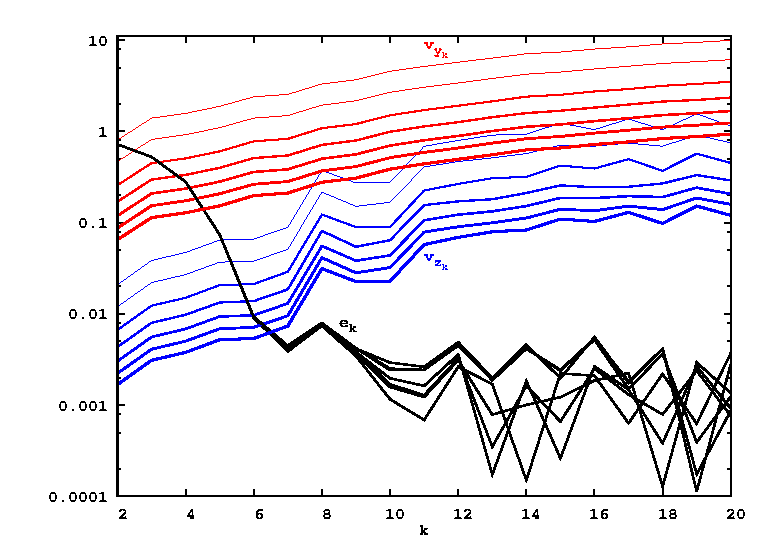
\includegraphics[width=3.5in]{fig_33_tube_cond_10_regularized_33_tube_k10_regularized_stab.eps}
\caption{
Culled volumes in the thin slice, single instance approximation of $\mat{s}^{-1/2}_{\tau_0 \mu_0}$
for the (3,3) nanotube, $\kappa(\mat{s})=10^{10}$ matrix series 
described in Section \ref{data}.  In the ``single'' instance, it was not possible to achieve stability with $\tau_0=.1$
In this ``single'' case, a thin slice corresponds to $\mu_0=.1, \tau_0=10^{-2} \;  \&  \; \tau_s=10^{-4}$, and volumes are
$\rm v_{\widetilde{\mat{z}_k}} = \left( {\rm vol}_{ \widetilde{\mat{z}}_{k-1}\ot h[\widetilde{\mat{x}}_{k-1}] } \right) \times 100\% /N^3$ and
${\rm v}_{\widetilde{\mat{y}}_k} = \left( {\rm vol}_{\mat{s}  \ots  \widetilde{\mat{z}}_{k}} \right) \times 100\% /N^3$.    
Line width increases with increasing system size. 
Also shown is the trace error, ${\rm e}_{k} = \left( N-{\rm tr}\,\mat{x}_k \right)/N$.}\label{regularized_stab}
\end{figure} 

\begin{figure}[h]
 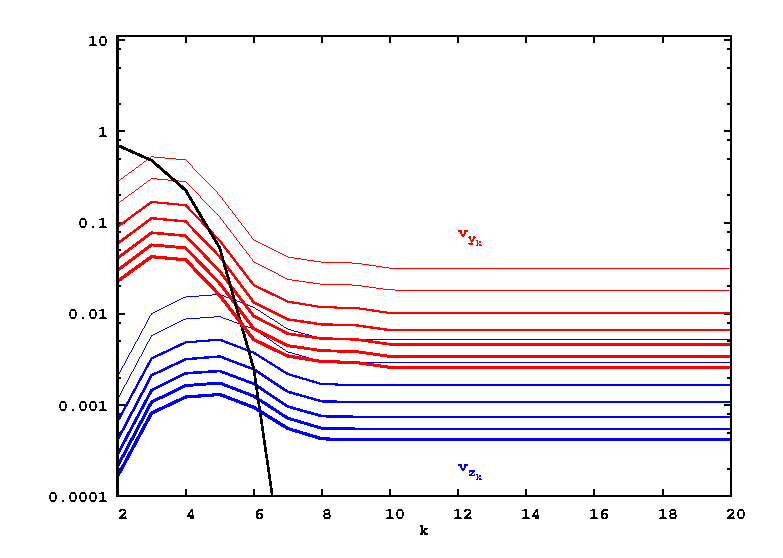
\includegraphics[width=3.5in]{fig_33_tube_cond_10_regularized_33_tube_k10_regularized_dual.eps}
% 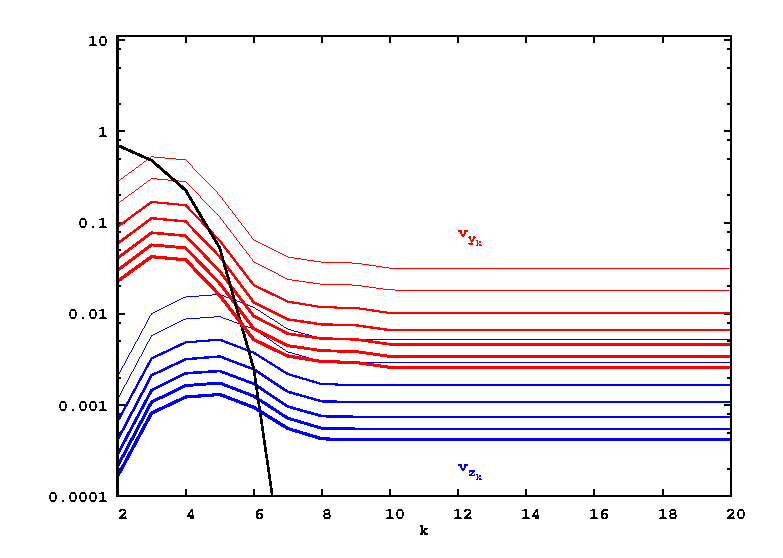
\includegraphics[width=3.5in]{fig_33_tube_cond_10_regularized/33_tube_k10_regularized_dual.eps}
\caption{
Culled volumes in the thin slice, dual instance approximation of $\mat{s}^{-1/2}_{\tau_0 \mu_0}$
for the (3,3) nanotube, $\kappa(\mat{s})=10^{10}$ matrix series 
described in Section \ref{data}. The thin slice corresponds to $\mu_0=.1, \tau_0=.1 \;  \&  \; \tau_s=.001$ 
with volumes 
${\rm v}_{\widetilde{\mat{y}}_k}= \left( {\rm vol}_{  h[\widetilde{\mat{x}}_{k-1}] \ots \widetilde{\mat{y}}_k }  \right) \times 100\% /N^3$ and  
${\rm v}_{\widetilde{\mat{z}}_k}= \left( {\rm vol}_{\widetilde{\mat{z}}_{k-1} \ot  h[\widetilde{\mat{x}}_{k-1}]} \right) \times 100\% /N^3$.
Line width increases with increasing system size. 
Also shown is the trace error, ${\rm e}_{k} = \left( N-{\rm tr}\,\mat{x}_k \right)/N$, which rapidly approaches $10^{-11}$ (not shown). 
}\label{regularized_dual}
\end{figure} 

% \begin{equation}\label{boundY}
% \Delta^{\mat{I}_{\tau_0 \mu_0} \cdot \mat{s}^{1/2}_{\tau_0 \mu_0}} <  \tau n \lVert \mat{s}^{1/2}_{\tau_0 \mu_0} \rVert
% \end{equation}
% and 
% \begin{equation}\label{boundZ}
% \Delta^{ \mat{s}^{-1/2}_{\tau_0 \mu_0}\cdot \mat{I}_{\tau_0 \mu_0}}  <  \tau n \lVert \mat{s}^{-1/2}_{\tau_0 \mu_0} \rVert \, ,
% \end{equation}

\subsection{Iterative regularization}

We now sketch an iterative approach to constructing the product representation, Eq.~(\ref{spammsandwich}).
In the dual instance, it is possible to obtain a first MAYEBOO approximation $\mat{s}^{-1/2}_{\tau_0={\tt .1}, \mu_0={\tt .1}}$,
which improves the condition number by one order of magnitude, with a numerical resolution of one digit.
Then, a next level slice can be found, $\mat{s}^{-1/2}_{\tau_0 \mu_1}$, based on the residual 
$\left(\mat{s}^{-1/2}_{\tau_0\mu_0} \right)^\dagger \, \otone \, \left(\mat{s}+\mu_1 \mat{I} \right)  
\, \otone \,\mat{s}^{-1/2}_{\tau_0 \mu_0} $, with {\em e.g.} 
$\mu_1= \tt .01$ and $\tau_1={\tt .01}$.   The product $\mat{s}^{-1/2}_{\tau_0 \mu_1}  \otone \mat{s}^{-1/2}_{\tau_0 \mu_0}$
then improves the condition number by two orders of magnitude, still with a numerical resolution of one digit.
In preliminary work, it appears necessary to compute the residual at a higher level of precision, 
{\em e.g.} using $\otone$ instead of $\oto$ and with $\tau_1 > \tau_0$.

In this way,  it may be possible to obtain product representation of the inverse square root at a $\tt SpAMM$ resolution that is
potentially far more permissive than otherwise possible,
\begin{equation} \label{product_rep}
\mat{s}^{-1/2}_{\tau_0} = \mat{s}^{-1/2}_{\tau_0 \mu_n} \, \otone \, \mat{s}^{-1/2}_{\tau_0 \mu_{n-1}} \, \otone \, \dots  \,  \mat{s}^{-1/2}_{\tau_0 \mu_0} \, ,
\end{equation}
assuming ${\tt .1} \ge \mu_0 > \mu_1 > \dots$  Likewise, it may also  be possible to obtain the full inverse factor with 
increasing numerical resolution as 
\begin{equation} \label{product_rep_tau}
\mat{s}^{-1/2} = \mat{s}^{-1/2}_{\tau_m} \, \otpm \,  \mat{s}^{-1/2}_{\tau_{m-1}} \, \otm \dots \, \mat{s}^{-1/2}_{\tau_0} \, ,
\end{equation}
and ${\tt .1} \ge  \tau_0 > \tau_1 > \dots $   

With each step a well conditioned generic slice, it may be possible to find a more effective logistic map optimized 
for the corresponding eigenvalue distributions. 
Also, there are  other paths that can be taken in the scoping of regularization and precision that
may be far more efficient. 

%Finally, our sketch is vague about our ability to avoid forming the 
%full product in application to a target vector or matrix.  

% As an example, we formalize the product representation (\ref{product_rep}) (a similar argument applies to (\ref{product_rep_tau}) and (\ref{spammsandwich})). To do so, let $\mu_{0}>\mu_{1}>\dots>\mu_{j}>0$, and suppose
% that, for $j\geq1$, $R_{j-1}$ is the $\tau_{0}$ approximation to
% $\left(S+\mu_{j-1}I\right)^{-1/2}$, so that 
% \[
% \left\Vert R_{j-1}^{\dagger}\otimes_{\tau_{0}}\left(S+\mu_{j-1}I\right)\otimes_{\tau_{0}}R_{j-1}-I\right\Vert _{F}\lesssim\tau_{0}.
% \]
% Now let $S_{\tau_{0},\mu_{j}}^{-1/2}$ denote a $\tau_{0}$ approximation
% to $R_{j-1}^{\dagger}\otimes_{\tau_{0}}\left(S+\mu_{j}I\right)\otimes_{\tau_{0}}R_{j-1}$.
% It follows that $R_{j}=R_{j-1}\otimes_{\tau_{0}}S_{\tau_{0},\mu_{j}}^{-1/2}$
% is a $\tau_{0}$ approximation to $\left(S+\mu_{j}I\right)^{-1/2}$. 
% Indeed, by the stability of SpAMM (\ref{bound}),
% \begin{eqnarray*}
% \left(R_{j-1}\otimes_{\tau_{0}}S_{\tau_{0},\mu_{j}}^{-1/2}\right)^{\dagger} & = & \left(R_{j-1}S_{\tau_{0},\mu_{j}}^{-1/2}\right)^{\dagger}+\mathcal{O}\left(\tau_{0}\right)\\
%  & = & \left(S_{\tau_{0},\mu_{j}}^{-1/2}\right)^{\dagger}\left(R_{j-1}\right)^{\dagger}+\mathcal{O}\left(\tau_{0}\right)\\
%  & = & \left(S_{\tau_{0},\mu_{j}}^{-1/2}\right)^{\dagger}\otimes_{\tau_{0}}\left(R_{j-1}\right)^{\dagger}+\mathcal{O}\left(\tau_{0}\right).
% \end{eqnarray*}
% Therefore,  \[
% \left\Vert R_{j}^{\dagger}\otimes_{\tau_{0}}\left(S+\mu_{j}I\right)\otimes_{\tau_{0}}R_{j}-I\right\Vert _{F}\lesssim\tau_{0},
% \]
% where $R_{j}$ is given by  the product representation
% \begin{eqnarray*}
% R_{j} & = & R_{j-1}\otimes_{\tau_{0}}S_{\tau_{0},\mu_{j}}^{-1/2}\\
%  & = & R_{j-2}\otimes_{\tau_{0}}S_{\tau_{0},\mu_{j-1}}^{-1/2}\otimes_{\tau_{0}}S_{\tau_{0},\mu_{j}}^{-1/2}\\
%  & = & S_{\tau_{0},\mu_{0}}^{-1/2}\otimes_{\tau_{0}}\dots\otimes_{\tau_{0}}S_{\tau_{0},\mu_{j-1}}^{-1/2}\otimes_{\tau_{0}}S_{\tau_{0},\mu_{j}}^{-1/2}.
% \end{eqnarray*}

%\begin{equation}
%\mat(I}\left(\mat{s}\right) = \bigotimes_{\substack{\tau=\tau_0 \\ \mu=\mu_0}}  \bigotimes_{\substack{\tau'=\tau_0 \\ \mu'=\mu_0}} 
%{_{\mat{s}^{1/2}} }{\left<\tau \mu \right|}
%{\left|\tau \mu \right>}_{\mat{s}^{-1/2}} 
%\end{equation}

%\pagebreak

\section{Locality} 


\begin{figure}[h] 
\fbox{ 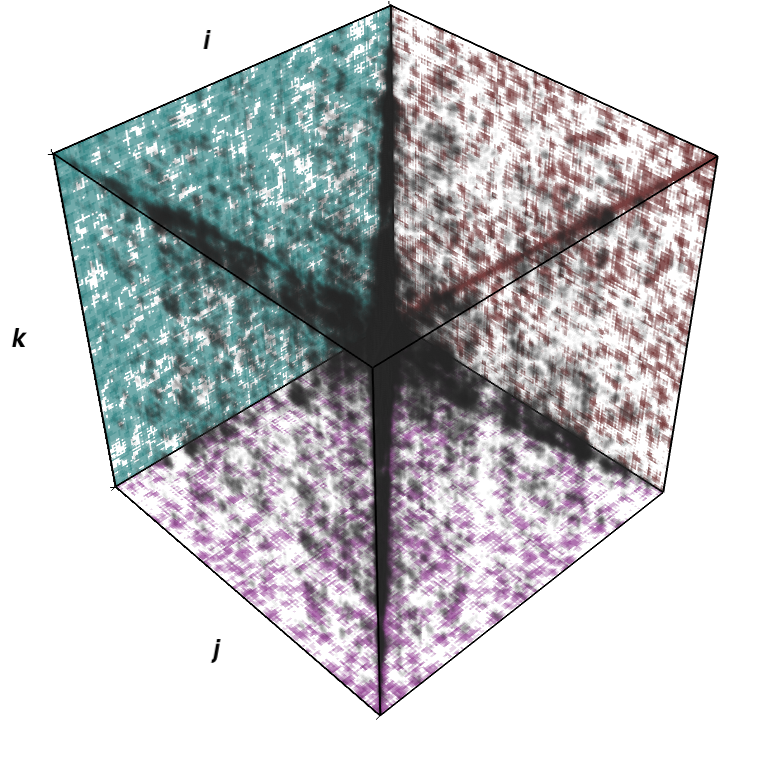
\includegraphics[width=2.45cm,keepaspectratio=true,
                       trim={0.cm 2.3cm 2.cm 1.cm},clip]
                       {fig_wtrbx_100_noregular_y_dual_0_cant_x.png}} 
%                       {fig_wtrbx_100_noregular/y_dual_0_cant_x.png}} 
\fbox{ 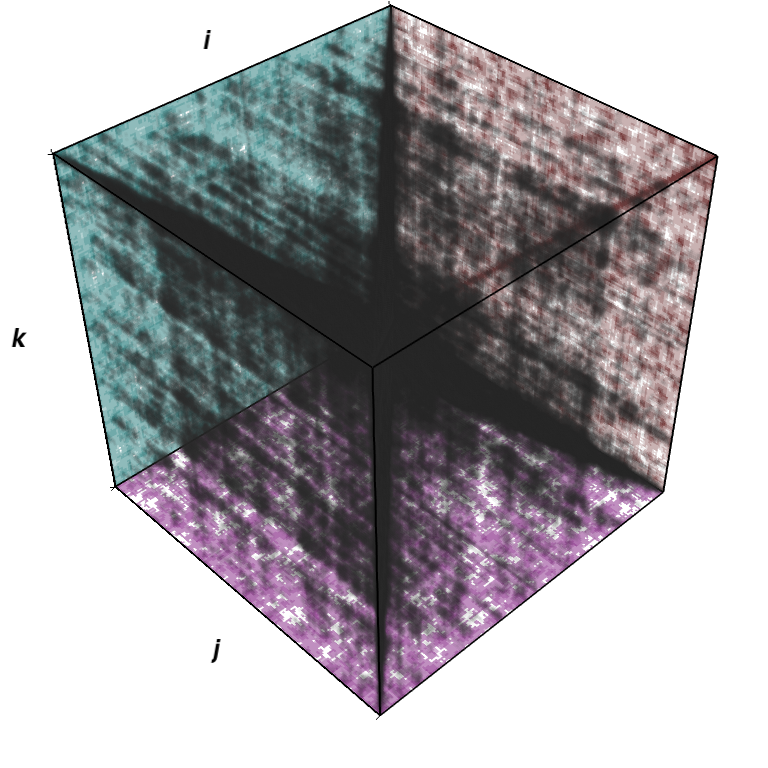
\includegraphics[width=2.45cm,keepaspectratio=true,
                        trim={0.cm 2.3cm 2.cm 1.cm},clip]
                        {fig_wtrbx_100_noregular_y_dual_5_cant_x.png}} 
%                        {fig_wtrbx_100_noregular/y_dual_5_cant_x.png}} 
\fbox{ 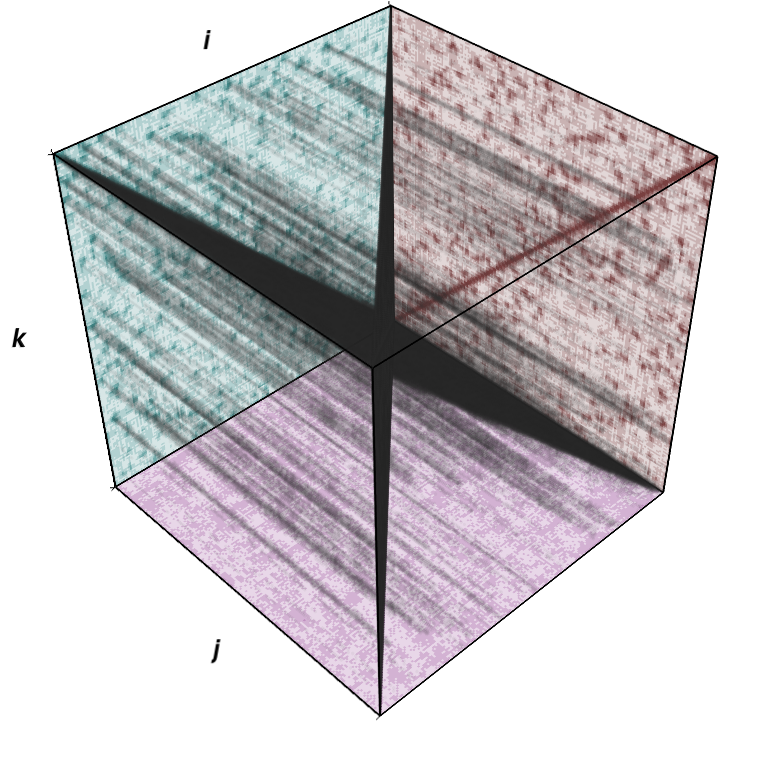
\includegraphics[width=2.45cm,keepaspectratio=true,
                        trim={0.cm 2.3cm 2.cm 1.cm},clip]
                        {fig_wtrbx_100_noregular_y_dual_17_cant_x.png}} 
%                        {fig_wtrbx_100_noregular/y_dual_17_cant_x.png}} 
\fbox{ 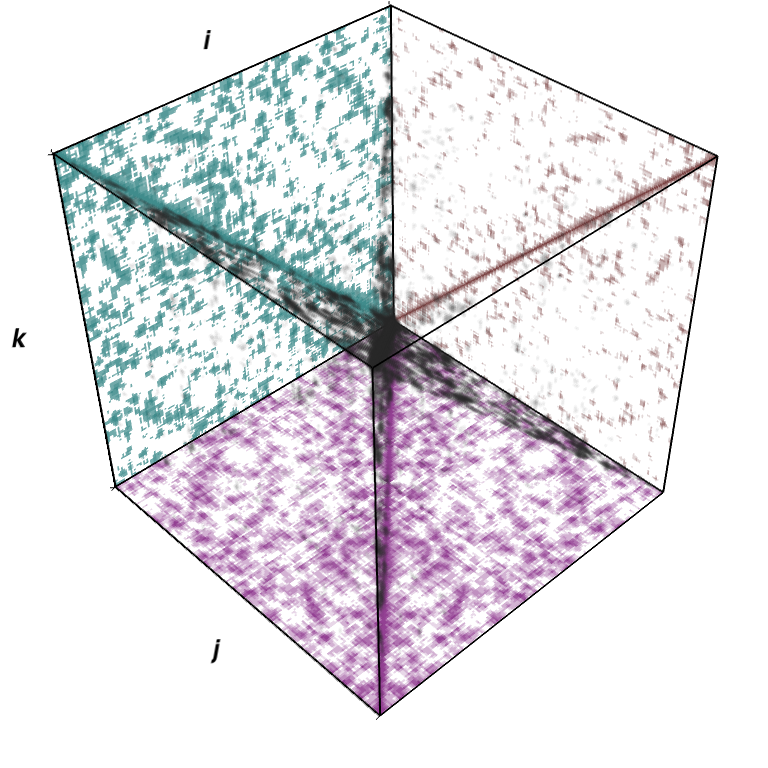
\includegraphics[width=2.45cm,keepaspectratio=true,
                        trim={0.cm 2.3cm 2.cm 1.cm},clip]
                        {fig_wtrbx_100_noregular_x_dual_0_cant_x.png}} 
%                        {fig_wtrbx_100_noregular/x_dual_0_cant_x.png}} 
\fbox{ 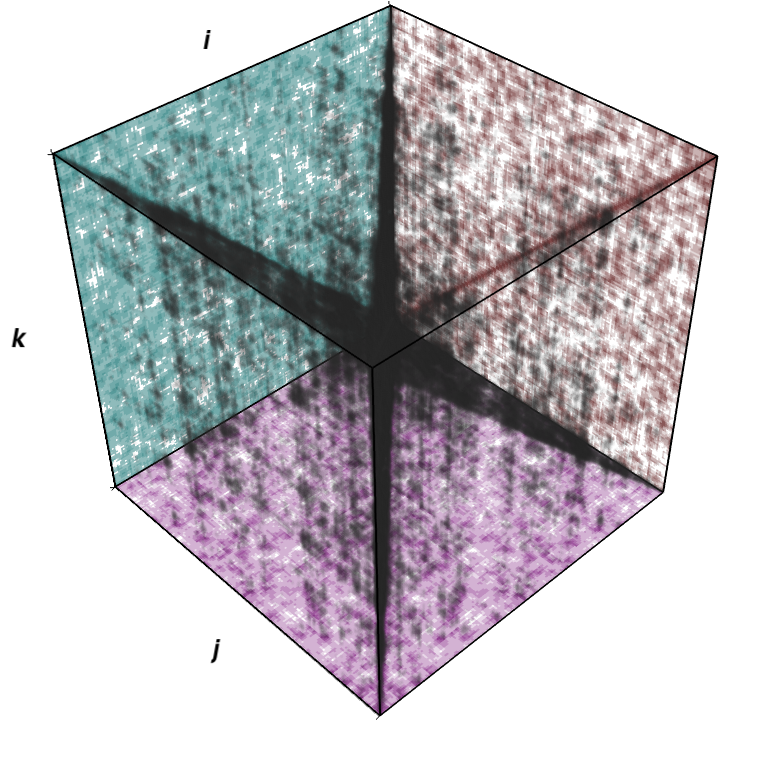
\includegraphics[width=2.45cm,keepaspectratio=true,
                        trim={0.cm 2.3cm 2.cm 1.cm},clip]
                        {fig_wtrbx_100_noregular_x_dual_5_cant_x.png}} 
%                        {fig_wtrbx_100_noregular/x_dual_5_cant_x.png}} 
\fbox{ 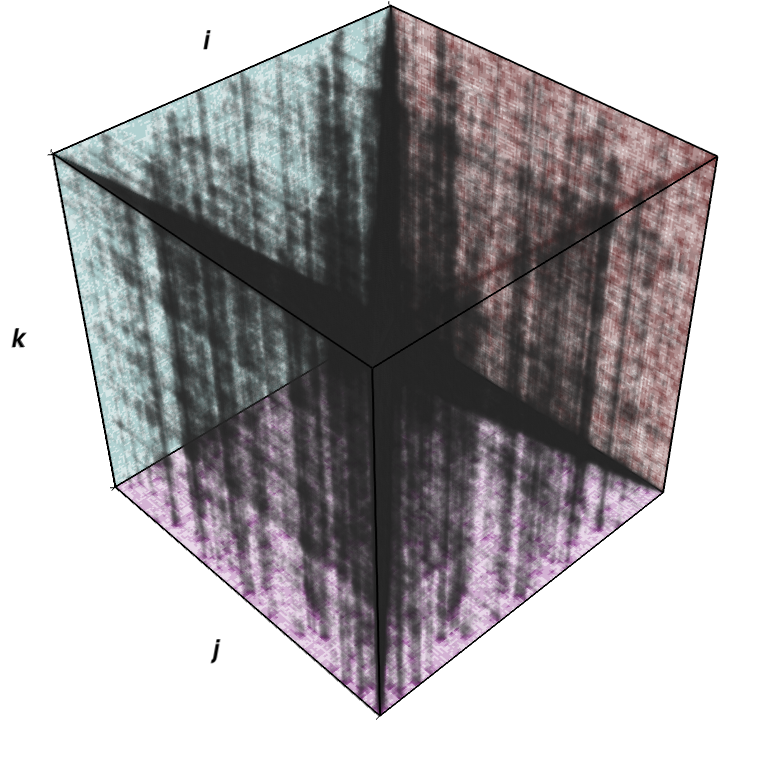
\includegraphics[width=2.45cm,keepaspectratio=true,
                        trim={0.cm 2.3cm 2.cm 1.cm},clip]
                        {fig_wtrbx_100_noregular_x_dual_17_cant_x.png}} 
%                        {fig_wtrbx_100_noregular/x_dual_17_cant_x.png}} 
\caption{
The $ijk$ task and data space for construction of the unregularized preconditioner 
$\left|\tau_0=.001,\mu_0=.0\, ; \,\scriptstyle{\mat{s}^{-1/2}} \right>$, with
dual instance square root iteration, and for the 6-311G** metric of 100 periodic water molecules
at STP.  At top its  $\mat{y}_k=h_\alpha[ \mat{x}_{k-1} ] \ots \mat{y}_{k-1}$
for $k=0,4,\& 15$, while on the bottom we have $\mat{x}_k=  \mat{y}_{k}  \ot \mat{z}_{k}$ for $k=0,4, \& 15$.
Maroon is $\mat{a}$, purple is $\mat{b}$, green is $\mat{c}$,  and black is the volume ${\rm vol}_{a \ot b}$
in the product $\mat{c}=\mat{a} \ot \mat{b}$.}\label{Lensing3}
\end{figure}

\subsection{Spatial, metric  and temporal locality}

Astrophysical $n$-body algorithms employ range queries over spatial databases to hierarchically discover 
and compute approximations that commit only small errors.  Often, these spatial databases are ordered with a 
space filling curve (SFC) 
\cite{Wise:1984:RMQ:1089389.1089398,springerlink:10.1007/3-540-51084-2_9,
      Samet:1990:DAS:77589,Wise1990,Wise:Ahnentafel,
      Lorton:2006:ABL:1166133.1166134,Samet:2006:DBDS,Adams:2006:SOS,Bock2013,bader13}, 
which maps points that are close in space to an index where they are also close. 
The block-by-magnitude structures empowering the $\tt SpAMM$ approximation are metric localities corresponding
to metric decay, in quantum chemical examples corresponding to an underlying SFC ordering of Carteisan coordinates. 

Warren and Salmon showed how to parlay spatial locality into temporal locality, 
remapping and repartitioning the space filling curve to rebalance distributed $n$-body tasks,
based on accumulated histories (persistence data).
In a similar way, we showed how persistence can be used to achieve 
strong parallel scaling for $\tt SpAMM$ with commonly available runtimes \cite{BockCK14}.  
Persistence data, providing temporal locality, may also be useful in mathematical approximation.  

%The locality of $\tt SpAMM$ volumes depends on opposing effects; ill-conditioning leads to delocalizations 
%and a broad spectral resolution, while strong metric seperation cooresponds to an increasing locality.  
%Unfortunately, seperation is diminished with increasing dimensionality.  

In Figure \ref{Lensing3}, we show $\ot$ volumes for square root iteration, corresponding to the metric of a small, periodic water box 
with the large 6-311G** basis (Appendix \ref{data}).  
For the 3-d periodic case, diminishing Cartesian separations lead to long-skinny delocalizations (pillae)
and much denser matrices, relative to {\em e.g.} a one-dimensional nano-tube.  

These delocalizations correspond to weakness in Eq.~(\ref{bound}),  
and to the tighter thresholds required to maintain a single iteration in the MAYSS approximation.  This effect is even more pronounced in the 
single instance (not shown), where delocalizations are exaggerated due to spectral resolutions that are broader.  
Eventually, Cartesian separation will thin the density of these delocalizations,  
with complexity reduction due to metric separation and decay only.  However, this may be painfully slow.  

\subsection{Algebraic locality}

In Figures \ref{Lensing1} and \ref{Lensing2},  we show a new kind of locality that is uniquely exploited by $n$-body approximation 
of the square root iteration.  This locality increases compressively towards convergence, 
as the contractive identity iteration develops.  
We call this compression {\bf  \em lensing},  involving collapse  of the culled volume about plane diagonals of the resolvent.
Lensing corresponds to strengthening Eq.(\ref{bound}), 
and to strongly contracting directional derivatives, Eqs.~(\ref{yorbit})-(\ref{zorbit}).
This is an important, mitigating computational effect for the sensitive $\mat{y}_k$ channel, 
with $\tau_s \sim {\tt .01} \times \tau$. 

In addition, non-Euclidean measures are relevant for achieving metric locality in 
the $\tt SpAMM$ algebra, including information measures, space filling curve generalizations, as well 
as graph reorderings that band matrix elements about the diagonal, a common approach in 
structural mechanics.   In Figure \ref{Lensing4} we show development of a first, unregularized (MAYSS) 
preconditioner for such an example; the structural matrix $\mat{s}={\tt bcsstk14}$ is a $\kappa(\mat{s})=10^{10}$ matrix 
corresponding to the roof of the Omni Coliseum in Atlanta.  These results show remarkable 
gossamer sheeting and flattening along plane diagonals, at top for development of $\mat{y}_k$, 
as well as hollow accumulation of ${\rm vol}_{\mat{y}_k \ot \mat{z}_k}$ at bottom.
Surprisingly, this example demonstrates lensing for a tight MAYSS approximation, while the 
equally ill-conditioned \& lower dimensional  $\kappa (\mat{s})=10^{10}$ nanotube MAYSS approximation 
remains full (dense) through U.C. $\times 128$.

\subsection{Complexity reduction}
  
Finally, we show complexity reduction at convergence of the MAYEBOO approximation relative to the MAYSS approximation, 
in Fig.~\ref{Complex1} for periodic water boxes, and in Fig.~\ref{Complex2} for the ill-conditioned nano-tube. 
The two-orders difference between $\mat{y}_k$ and $\mat{z}_k$ volumes corresponds precisely to $\tau_s \sim \tau \times {\tt .01}$, 
with $\mat{x}_k$ in between. Except for the slower trend in Fig.~(\ref{Complex1})'s $\mat{x}_k$ volume, we see the 
potential for continued strong acceleration with increasing system size.  Understanding these subtleties is the subject of future work. 

\begin{figure}[tb] 
\fbox{ 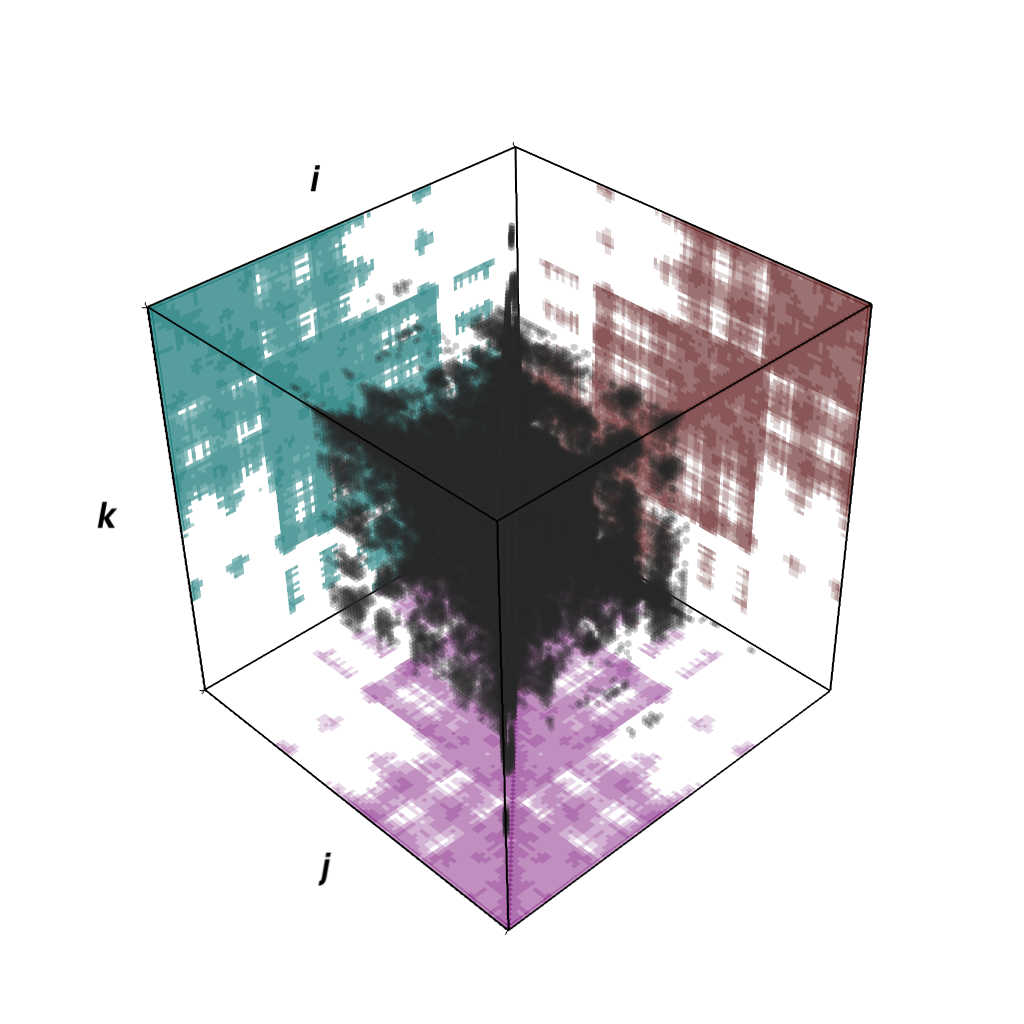
\includegraphics[width=2.45cm,keepaspectratio=true,
                        trim={3.cm 3.cm 5.cm 5.cm},clip]
                        {fig_33_8x_tube_cond_10_dual_thin_slices_y_dual_0_cant_x.png}} 
%                        {fig_33_8x_tube_cond_10_dual_thin_slices/y_dual_0_cant_x.png}} 
\fbox{ 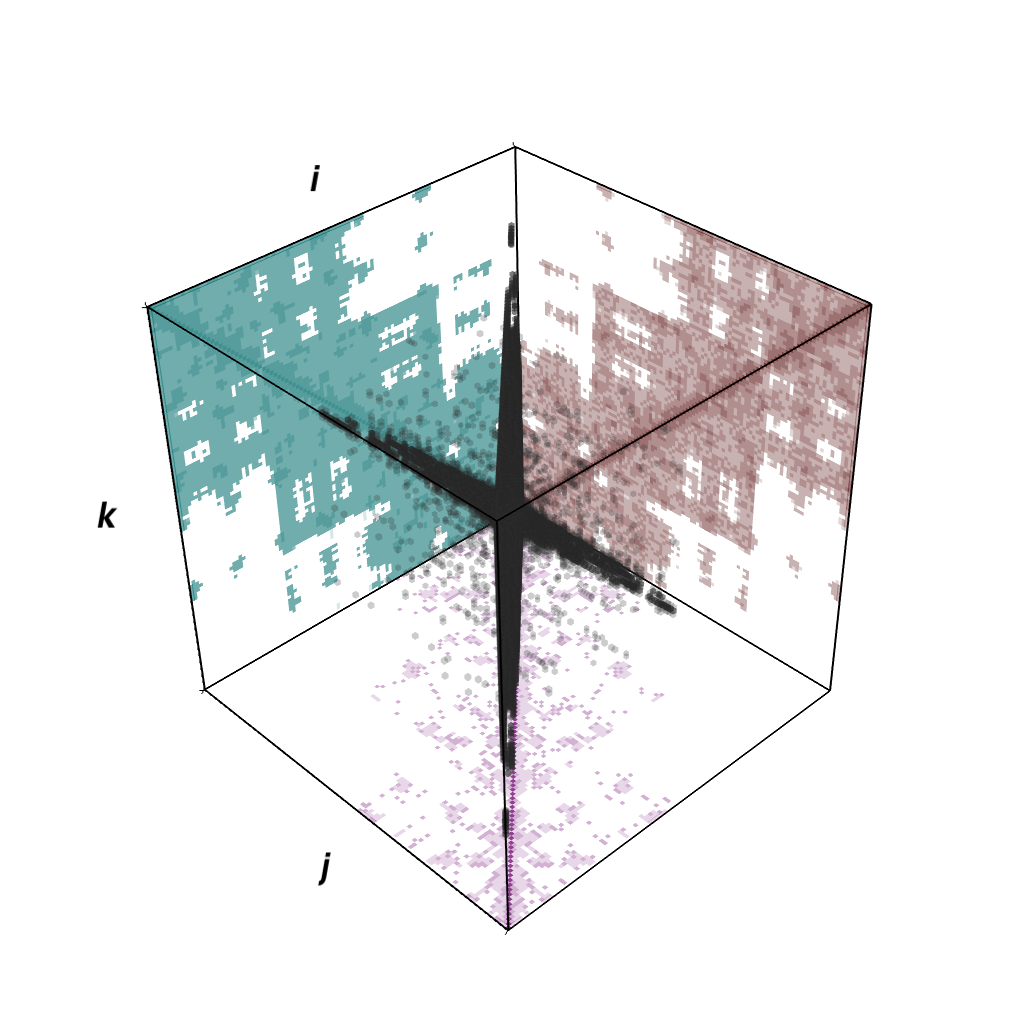
\includegraphics[width=2.45cm,keepaspectratio=true,
                        trim={3.cm 3.cm 5.cm 5.cm},clip]
                        {fig_33_8x_tube_cond_10_dual_thin_slices_y_dual_4_cant_x.png}} 
%                        {fig_33_8x_tube_cond_10_dual_thin_slices/y_dual_4_cant_x.png}} 
\fbox{ 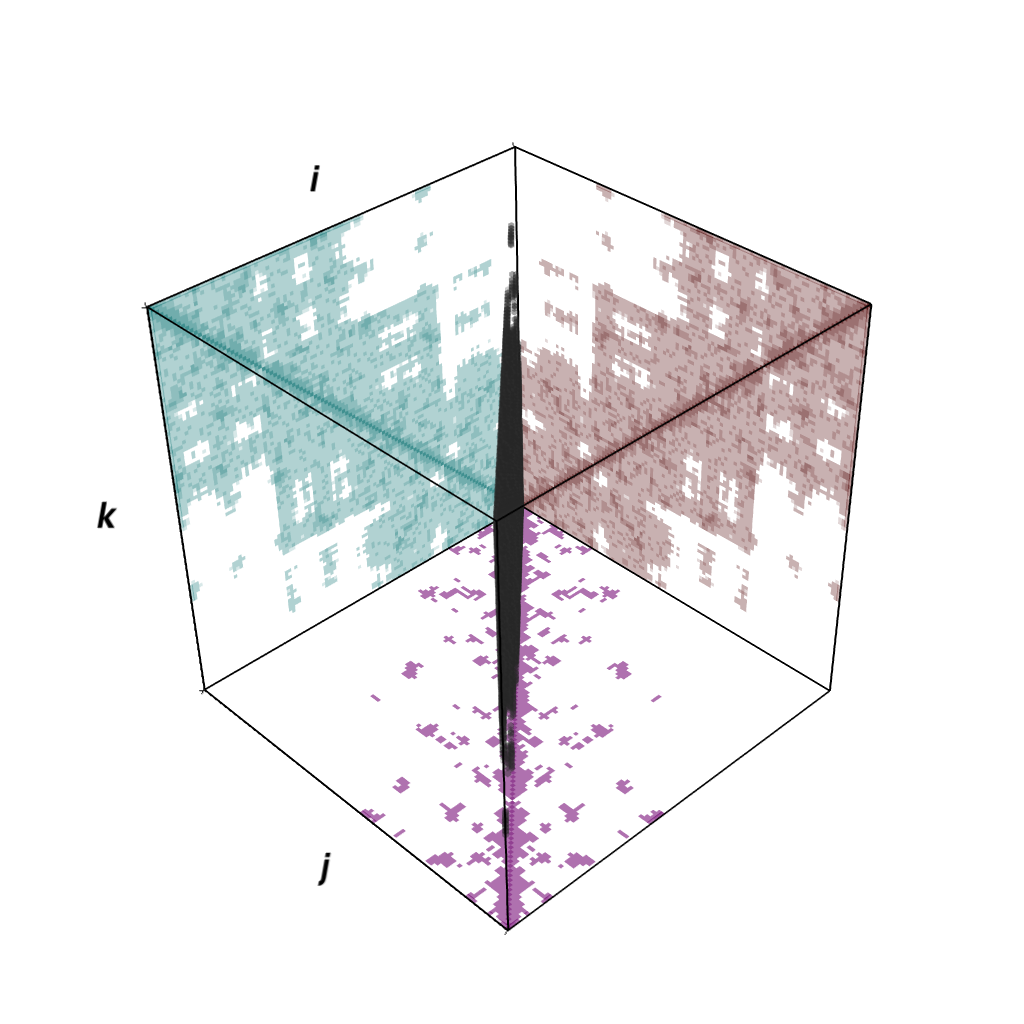
\includegraphics[width=2.45cm,keepaspectratio=true,
                        trim={3.cm 3.cm 5.cm 5.cm},clip]
                        {fig_33_8x_tube_cond_10_dual_thin_slices_y_dual_16_cant_x.png}} 
%                        {fig_33_8x_tube_cond_10_dual_thin_slices/y_dual_16_cant_x.png}} 
\fbox{ 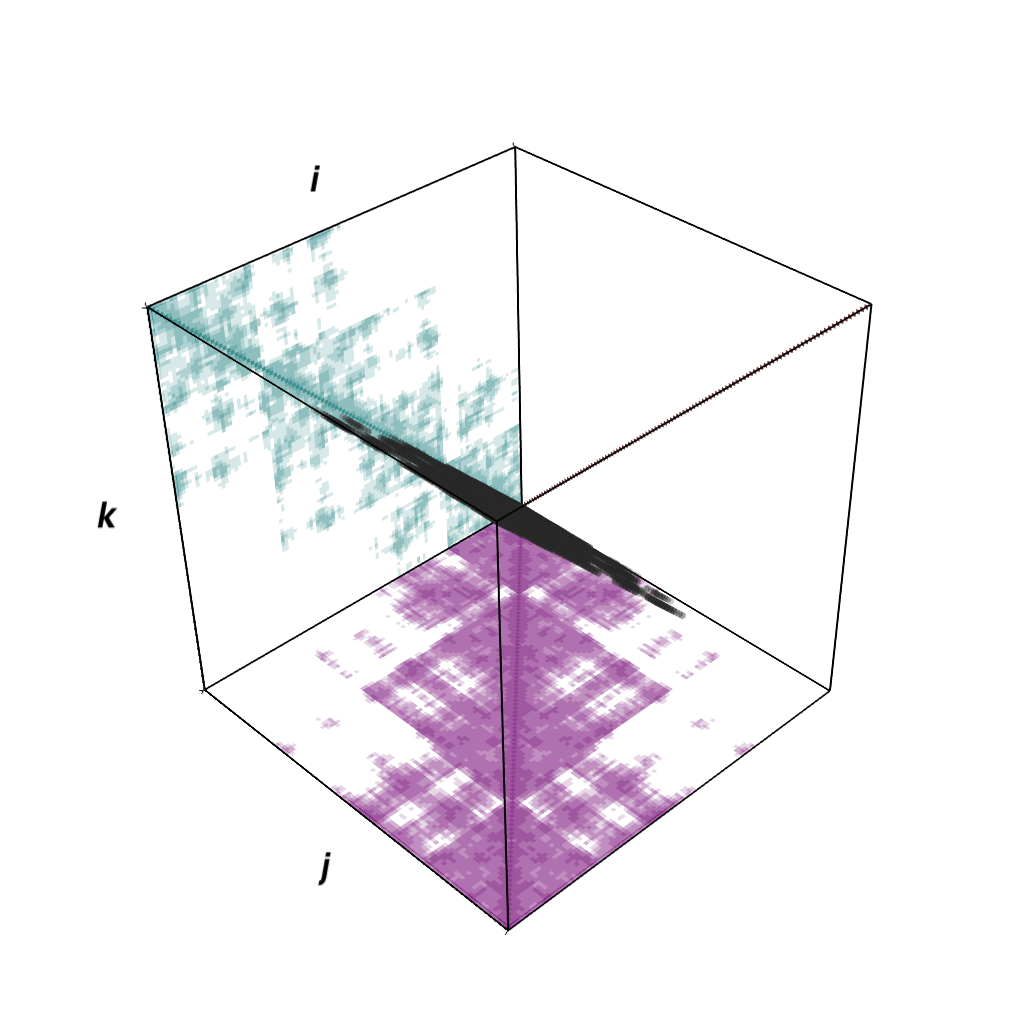
\includegraphics[width=2.45cm,keepaspectratio=true,
                        trim={3.cm 3.cm 5.cm 5.cm},clip]
                        {fig_33_8x_tube_cond_10_dual_thin_slices_x_dual_0_cant_x.png}} 
%                        {fig_33_8x_tube_cond_10_dual_thin_slices/x_dual_0_cant_x.png}} 
\fbox{ 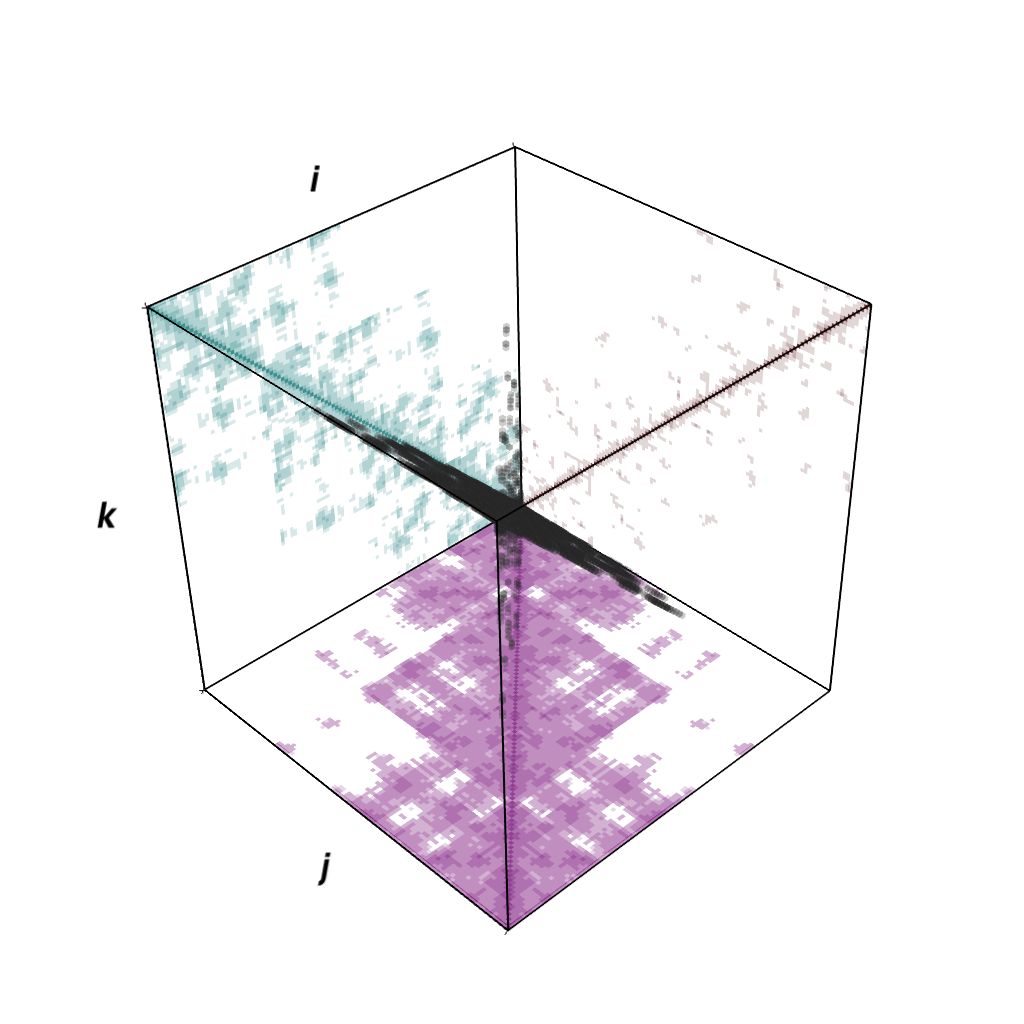
\includegraphics[width=2.45cm,keepaspectratio=true,
                        trim={3.cm 3.cm 5.cm 5.cm},clip]
                        {fig_33_8x_tube_cond_10_dual_thin_slices_x_dual_2_cant_x.png}} 
%                        {fig_33_8x_tube_cond_10_dual_thin_slices/x_dual_2_cant_x.png}} 
\fbox{ 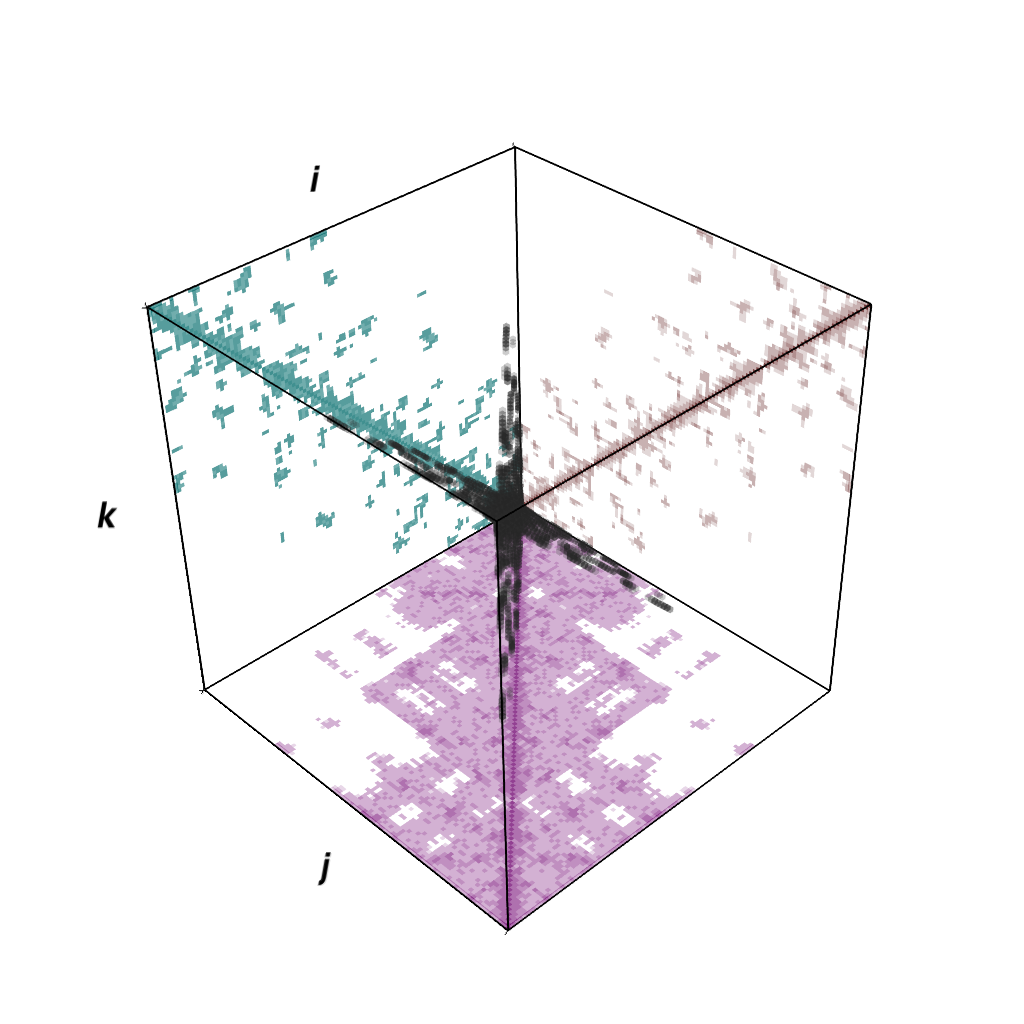
\includegraphics[width=2.45cm,keepaspectratio=true,
                        trim={3.cm 3.cm 5.cm 5.cm},clip]
                        {fig_33_8x_tube_cond_10_dual_thin_slices_x_dual_16_cant_x.png}} 
%                        {fig_33_8x_tube_cond_10_dual_thin_slices/x_dual_16_cant_x.png}} 
\caption{
The $ijk$ task and data space for construction of the MAYEBOO preconditioner 
$\left|\tau_0=.1,\mu_0=.1\, ; \,\scriptstyle{\mat{s}^{-1/2}} \right>$, with 
dual instance square root iteration,  and for an 8$\times$ U.C. (3,3) $\kappa(s)=10^{11}$ nanotube.
$\mat{y}_k$ appears wider than $\mat{z}_k$ because it is computed at a higher precision, $\tau_s=.001$,
and because the first multiply involves $\mat{s}^2$.  At top its  $\mat{y}_k=h_\alpha[ \mat{x}_{k-1} ] \ots \mat{y}_{k-1}$
for $k=0,4,\& 16$, while on the bottom we have $\mat{x}_k=  \mat{y}_{k}  \ot \mat{z}_{k}$ for $k=0,2, \& 16$.
Maroon is $\mat{a}$, purple is $\mat{b}$, green is $\mat{c}$,  and black is the volume ${\rm vol}_{a \ot b}$
in the product $\mat{c}=\mat{a} \ot \mat{b}$.}\label{Lensing1}
\end{figure}


\begin{figure}[tb] 
\fbox{ 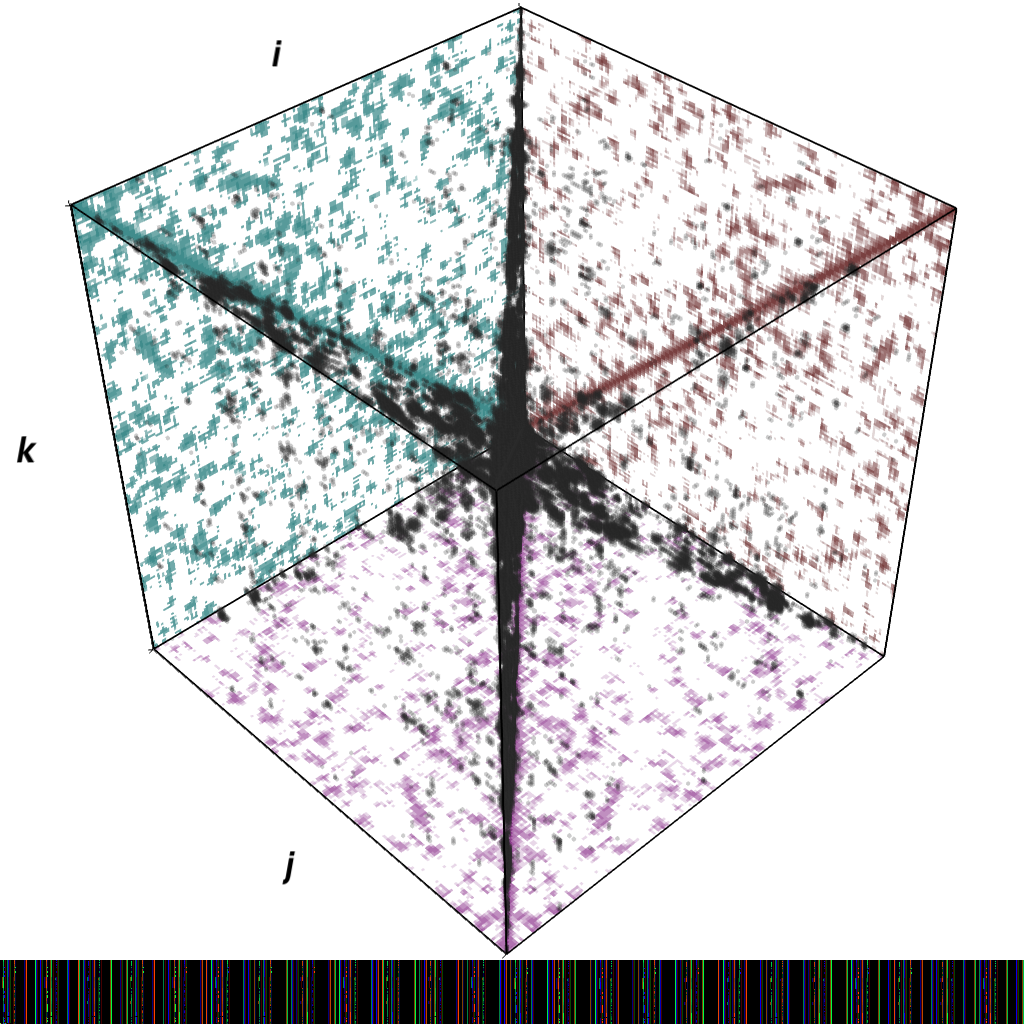
\includegraphics[width=2.45cm,keepaspectratio=true,
                       trim={0.cm 2.3cm 2.cm 1.cm},clip]
                       {fig_wtrbx_100_regularized_y_dual_0_cant_x.png}} 
%                       {fig_wtrbx_100_regularized/y_dual_0_cant_x.png}} 
\fbox{ 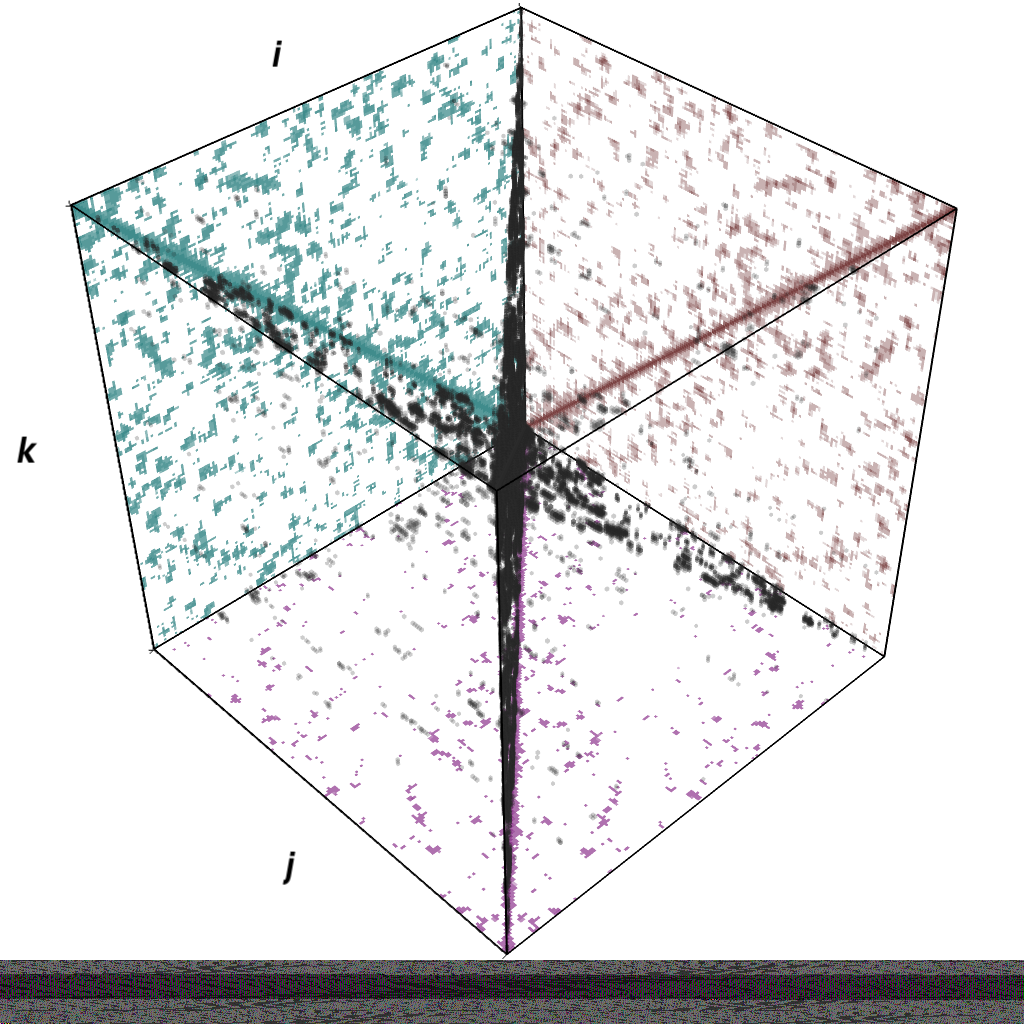
\includegraphics[width=2.45cm,keepaspectratio=true,
                        trim={0.cm 2.3cm 2.cm 1.cm},clip]
                        {fig_wtrbx_100_regularized_y_dual_4_cant_x.png}} 
%                        {fig_wtrbx_100_regularized/y_dual_4_cant_x.png}} 
\fbox{ 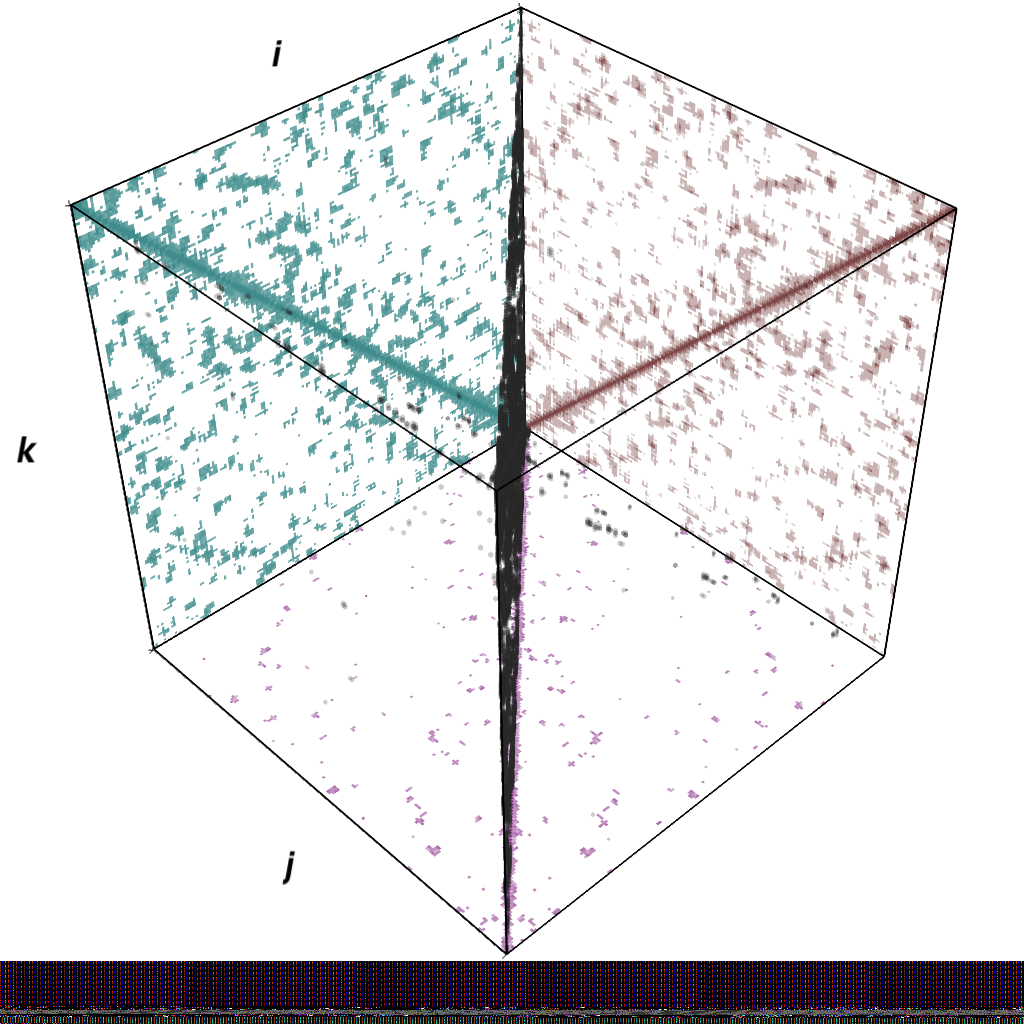
\includegraphics[width=2.45cm,keepaspectratio=true,
                        trim={0.cm 2.3cm 2.cm 1.cm},clip]
                        {fig_wtrbx_100_regularized_y_dual_15_cant_x.png}} 
%                        {fig_wtrbx_100_regularized/y_dual_15_cant_x.png}} 
\fbox{ 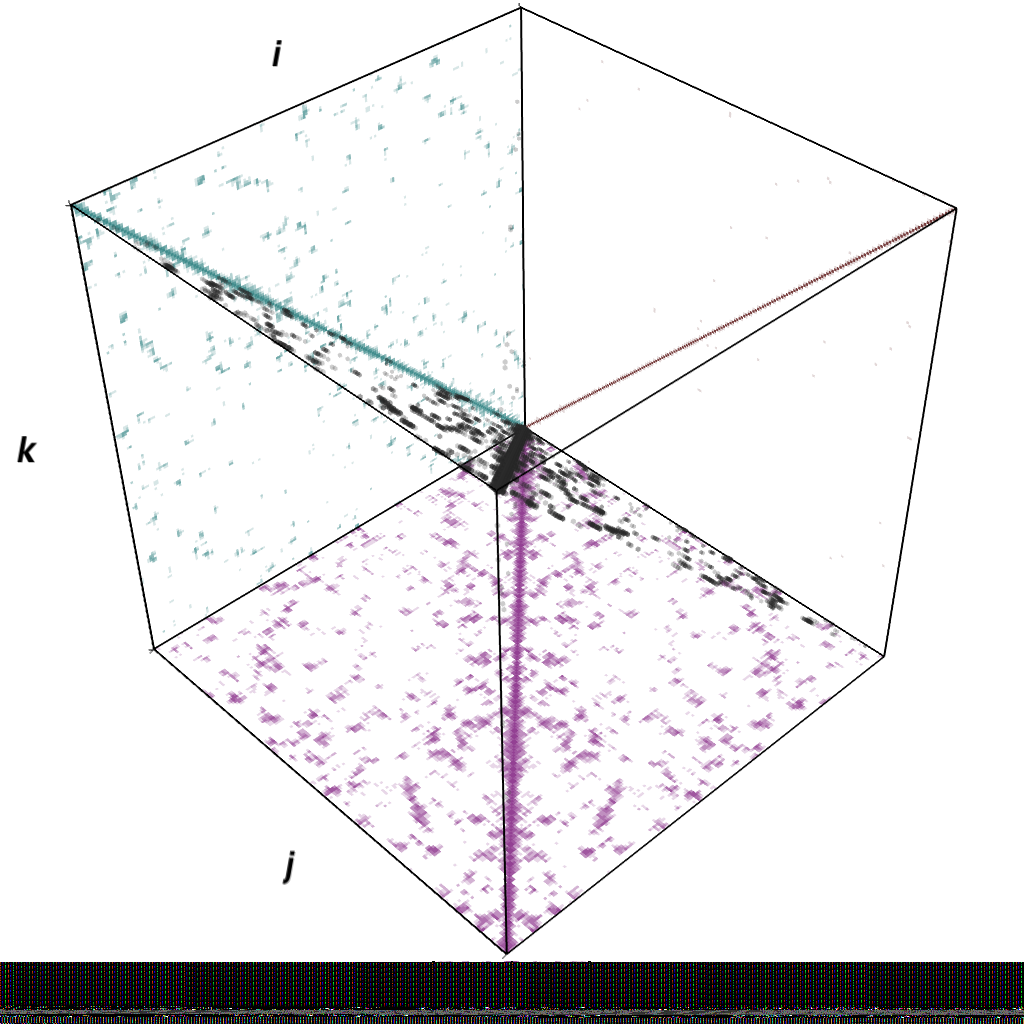
\includegraphics[width=2.45cm,keepaspectratio=true,
                        trim={0.cm 2.3cm 2.cm 1.cm},clip]
                        {fig_wtrbx_100_regularized_x_dual_0_cant_x.png}} 
%                        {fig_wtrbx_100_regularized/x_dual_0_cant_x.png}} 
\fbox{ 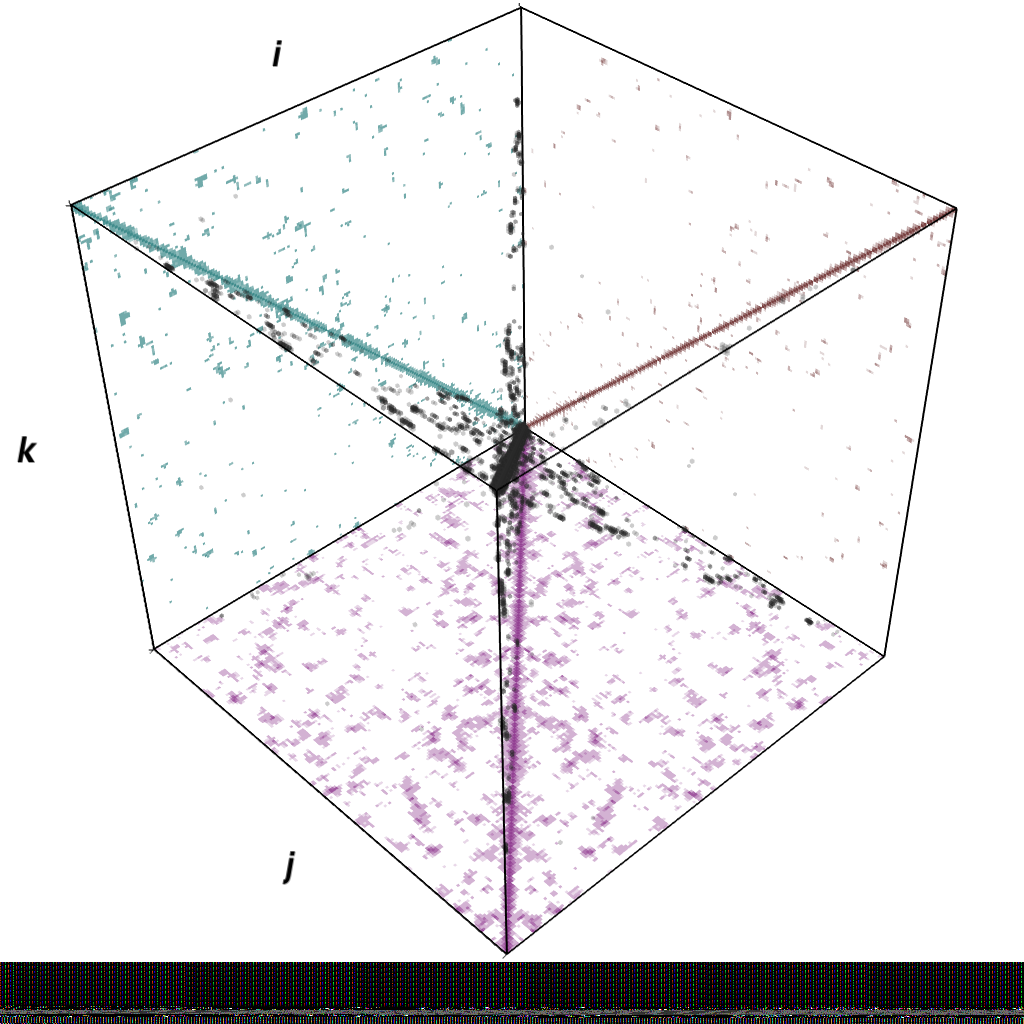
\includegraphics[width=2.45cm,keepaspectratio=true,
                        trim={0.cm 2.3cm 2.cm 1.cm},clip]
                        {fig_wtrbx_100_regularized_x_dual_4_cant_x.png}} 
%                        {fig_wtrbx_100_regularized/x_dual_4_cant_x.png}} 
\fbox{ 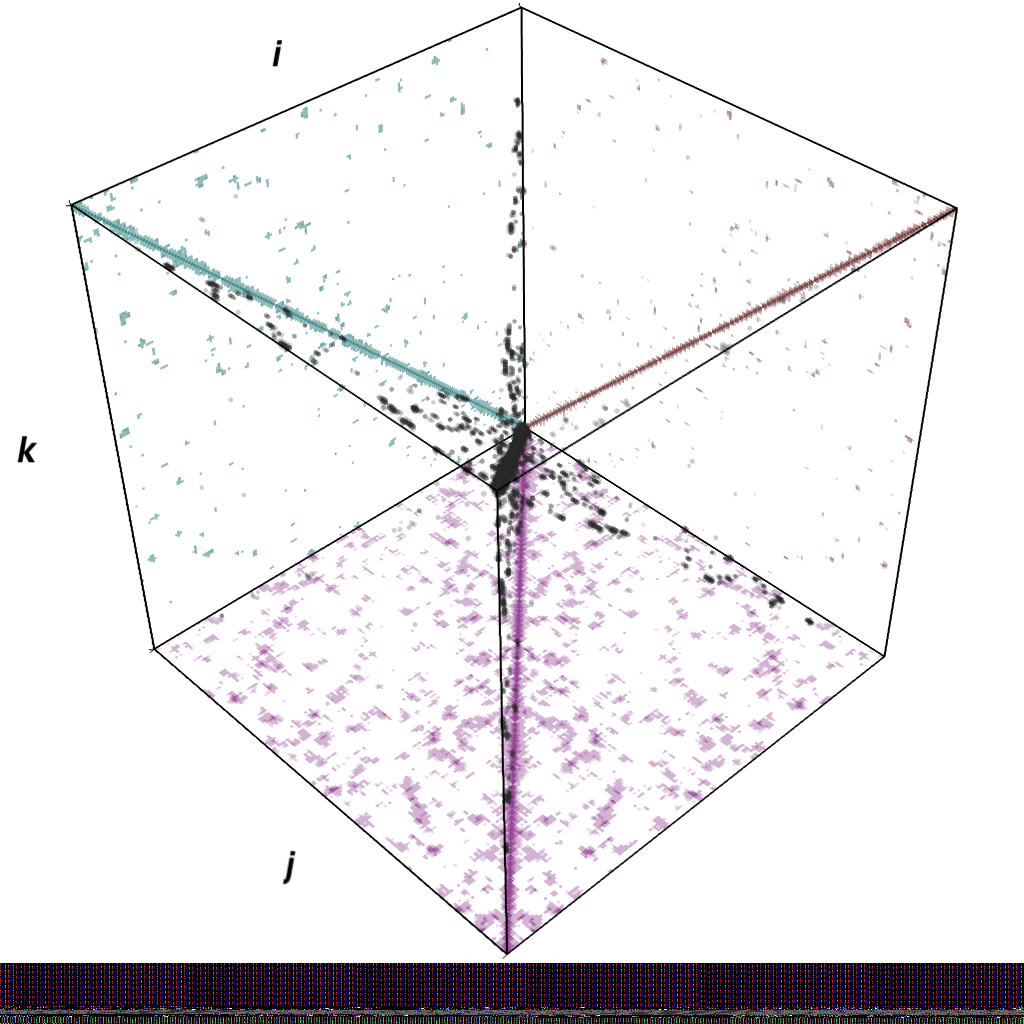
\includegraphics[width=2.45cm,keepaspectratio=true,
                        trim={0.cm 2.3cm 2.cm 1.cm},clip]
                        {fig_wtrbx_100_regularized_x_dual_15_cant_x.png}} 
%                        {fig_wtrbx_100_regularized/x_dual_15_cant_x.png}} 
\caption{
The $ijk$ task and data space for construction of the MAYEBOO preconditioner 
$\left|\tau_0=.1,\mu_0=.1\, ; \,\scriptstyle{\mat{s}^{-1/2}} \right>$, with 
dual instance square root iteration  and for 6-311G** metric of 100 periodic water molecules
at STP.  At top its  $\mat{y}_k=h_\alpha[ \mat{x}_{k-1} ] \ots \mat{y}_{k-1}$
for $k=0,4,\& 15$, while on the bottom we have $\mat{x}_k=  \mat{y}_{k}  \ot \mat{z}_{k}$ for $k=0,4, \& 15$.
Maroon is $\mat{a}$, purple is $\mat{b}$, green is $\mat{c}$,  and black is the volume ${\rm vol}_{a \ot b}$
in the product $\mat{c}=\mat{a} \ot \mat{b}$.}\label{Lensing2}
\end{figure}

\begin{figure}[tb] 
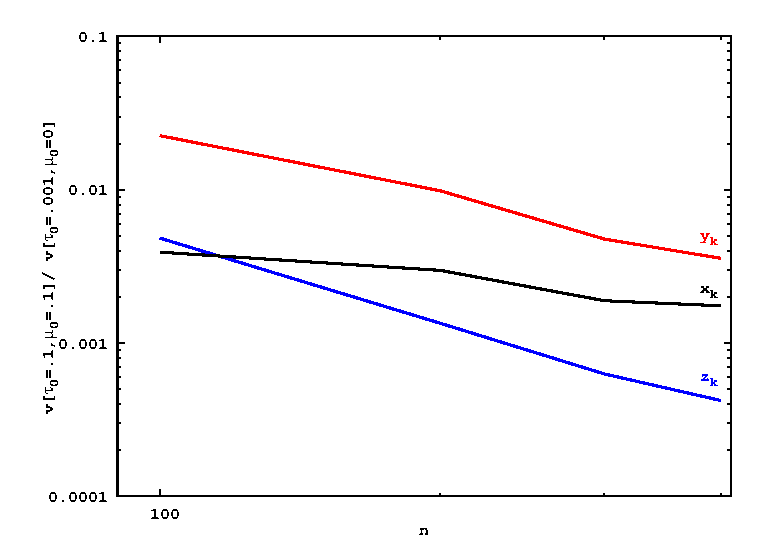
\includegraphics[width=7.8cm,keepaspectratio=true,trim={0.cm 0.cm 0.cm 0.cm},clip]
                 {fig_regular_and_unleaded_pcnt_volume_water_boxes.eps} 
%                 {fig_regular_and_unleaded/pcnt_volume_water_boxes.eps} 
\caption{ 
Complexity reduction in metric square root iteration for periodic 6-311G** water. 
Shown is the ratio of lensed product volumes for the regularized most-approximate-yet-effective-by-one-order (MAYEBOO) 
approximation and the unregularized most-approximate-yet-still-stable (MAYSS) approximation.}\label{Complex1}
\end{figure}

\begin{figure}[tb] 
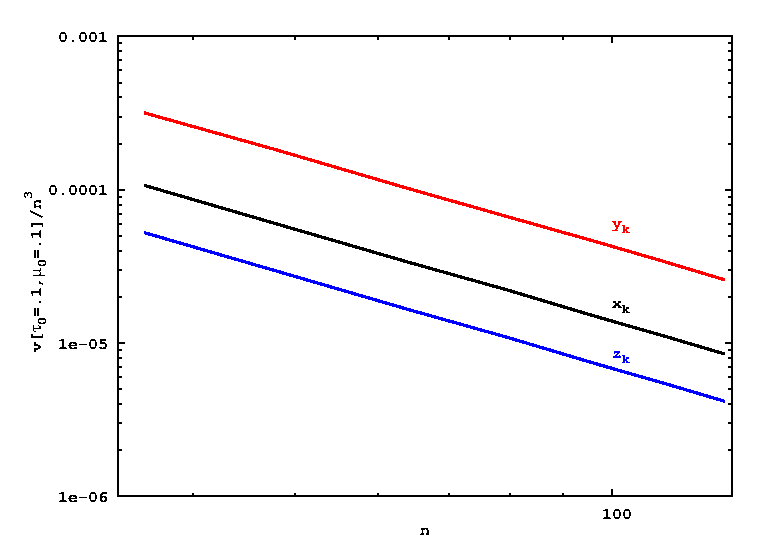
\includegraphics[width=7.8cm,keepaspectratio=true,trim={0.cm 0.cm 0.cm 0.cm},clip]
                 {fig_33_tube_cond_10_regularized_volume_vs_n3_tubes.eps} 
%                 {fig_33_tube_cond_10_regularized/volume_vs_n3_tubes.eps} 
\caption{ 
Complexity reduction in metric square root iteration for periodic 6-311G** water. 
Shown is the ratio of lensed product volumes for the regularized most-approximate-yet-effective-by-one-order (MAYEBOO) 
approximation and the unregularized most-approximate-yet-still-stable (MAYSS) approximation.}\label{Complex2}
\end{figure}


\begin{figure}[tb] 
\fbox{ 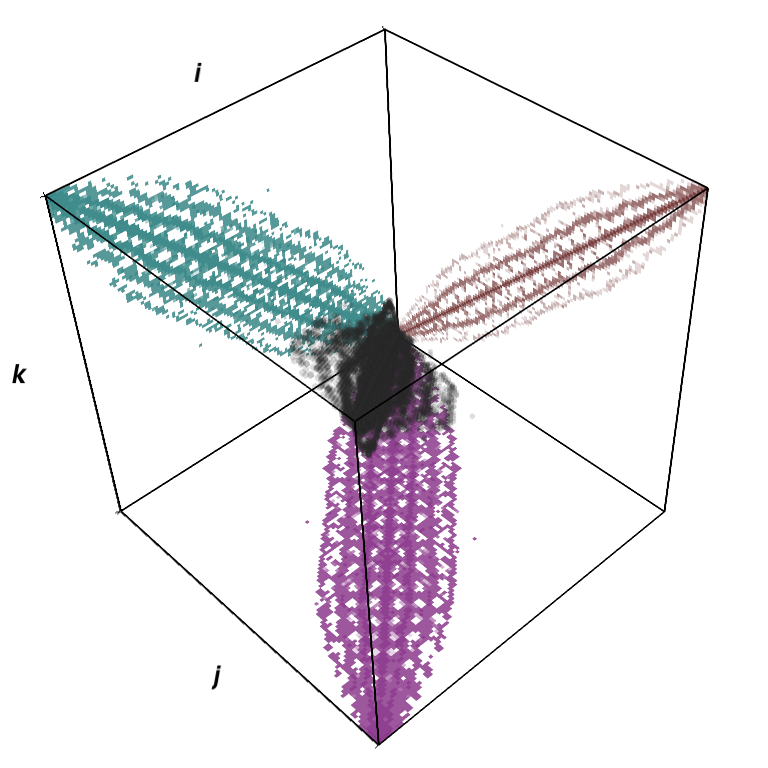
\includegraphics[width=3.8cm,keepaspectratio=true,
                        trim={0.cm 2.3cm 2.cm 1.cm},clip]
                        {fig_bcsstk14_y_dual_14_cant_x.png}} 
%                        {fig_bcsstk14/y_dual_14_cant_x.png}} 
\fbox{ 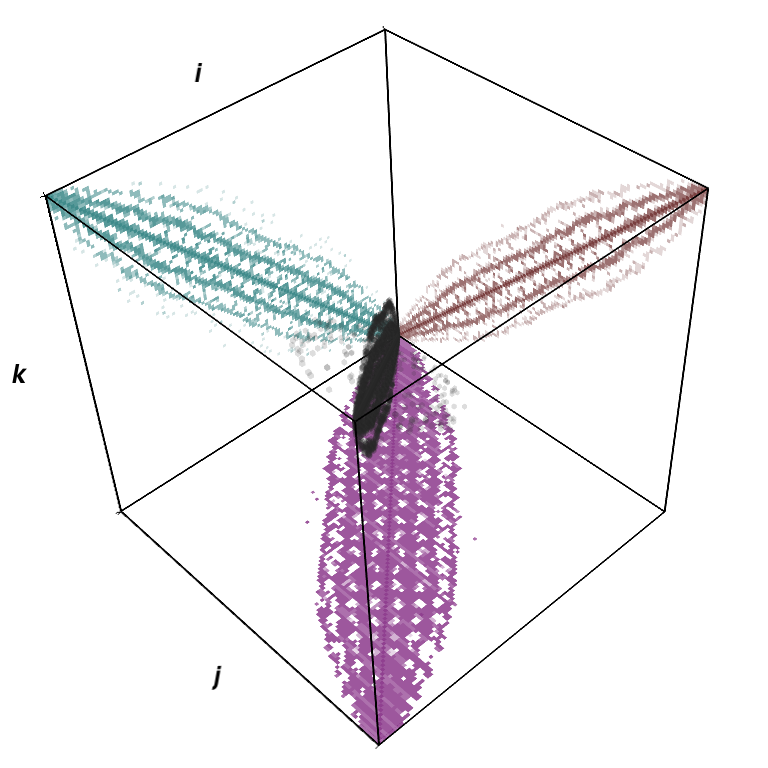
\includegraphics[width=3.8cm,keepaspectratio=true,
                        trim={0.cm 2.3cm 2.cm 1.cm},clip]
                        {fig_bcsstk14_y_dual_37_cant_x.png}} 
%                        {fig_bcsstk14/y_dual_37_cant_x.png}} 
\fbox{ 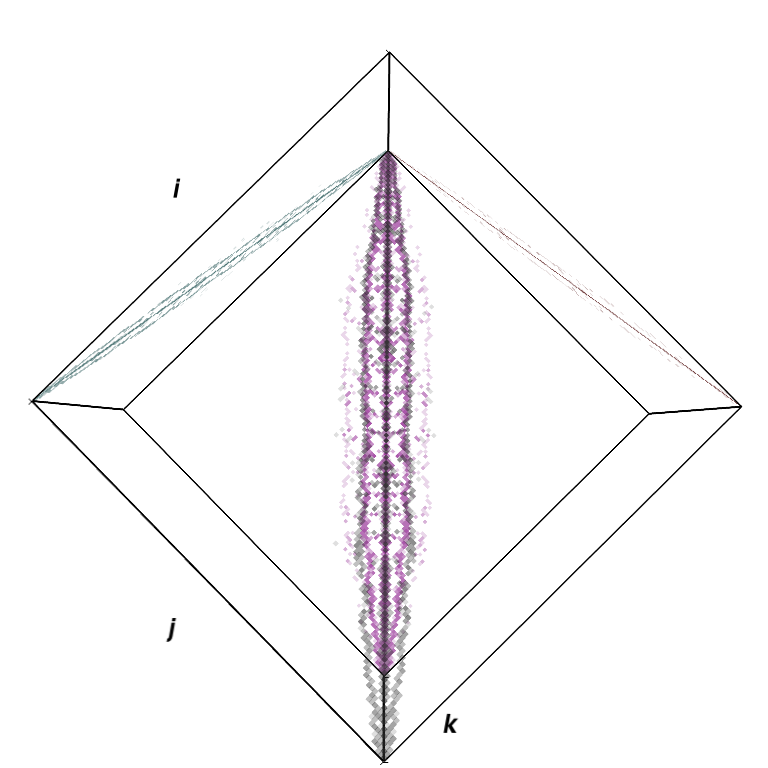
\includegraphics[width=3.8cm,keepaspectratio=true,
                        trim={0.cm 2.3cm 2.cm 1.cm},clip]
                        {fig_bcsstk14_x_dual_0_cant_x2.png}} 
%                        {fig_bcsstk14/x_dual_0_cant_x2.png}} 
\fbox{ 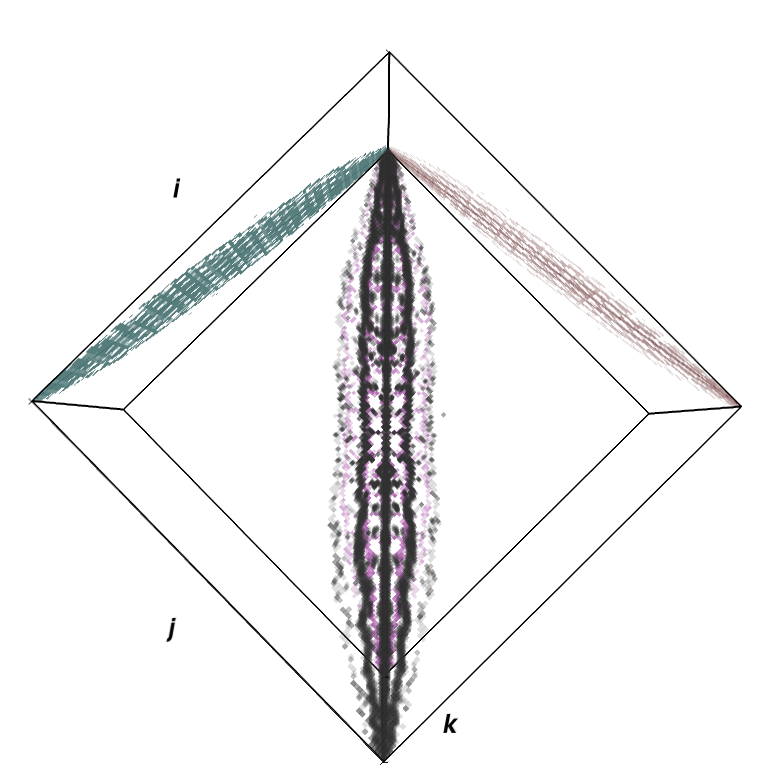
\includegraphics[width=3.8cm,keepaspectratio=true,
                        trim={0.cm 2.3cm 2.cm 1.cm},clip]
                        {fig_bcsstk14_x_dual_37_cant_x2.png}} 
%                        {fig_bcsstk14/x_dual_37_cant_x2.png}} 
\caption{
The $ijk$ task and data space for construction of the unregularized preconditioner 
$\left|\tau_0=.001,\mu_0=.0\, ; \,\scriptstyle{\mat{s}^{-1/2}} \right>$, with the 
dual instance of square root iteration  and for 6-311G** metric of 100 periodic water molecules
at STP.  At top its  $\mat{y}_k=h_\alpha[ \mat{x}_{k-1} ] \ots \mat{y}_{k-1}$
for $k=0,4,\& 15$, while on the bottom we have $\mat{x}_k=  \mat{y}_{k}  \ot \mat{z}_{k}$ for $k=0,4, \& 15$.
Maroon is $\mat{a}$, purple is $\mat{b}$, green is $\mat{c}$,  and black is the volume ${\rm vol}_{a \ot b}$
in the product $\mat{c}=\mat{a} \ot \mat{b}$.}\label{Lensing4}
\end{figure}

%The $n$-body solver carries out metric querries with occlusion-culling based on 
%with a bounded relative error in the product, given by Eq.~\ref{}. 
%$\tt SpAMM$ expoits metric locality, cooresponding to decay with Cartesian or non-Euclidian seperation, 
%and also algebraic locality, developing with identity iteration.  
%The $\tt SpAMM$ querry hierarchically resolves complex algebraic structures in the product space of square root iteration,  
%culling out the $i=k$ and $i=k$ planes and along the $ijk$ cube-diagonal.  In the case of the dual $\mat{y}_k$ and $\mat{z}_k$ channels,  
%these structures contract further as multiplication by near-identity is reached, with
%{\em lensing} about the plane diagonal and computational complexities tending towards quadtree-copy-in-place.

% \section{Summary}
% In this work, we developed the $n$-body solver $\tt SpAMM$ for square root iteration.   
% Main contributions include a modified Cauchy-Schwarz criterion, Eq.~\ref{}, and proof that the 
% cooresponding relative product error is bound by Eq.~(\ref{bound}).  Also, we demonstrated a new kind of 
% algebraic locality, {lensing}, that develops with strongly contractive identity iteration.
 
% In Section \ref{}, we looked at stability leading to the basin of convergence and sensitivity of the three
% product channels $\mat{y}_k$, $\mat{z}_k$ and $\mat{x}_k$, for the $\tt SpAMM$ approximation in the 
% cannonical ``dual'' instance, Eq.~(\ref{}), and for the ``single'' instance, Eq.~(\ref{}).
% Consistent with HMMT \cite{}, the $\mat{z}_k$ channel is sensitized by the full inverse,
% $\mat{s}^{-1}$, requiring a tighter threshold for that case, $\tau_s \ll \tau$.  Later, we find that 
% extra cost is strongly mitigated by lensing.  Also in Section \ref{}, we looked at bifurcations 
% of scaled and unscaled iterations for ill-conditioned systems, towards a most-approximate-yet-still-stable (MAYSS) 
% preconditioner, and disected competing effects at the edge of stability,  between compounding displacement magnitudes and 
% strongly convergent directional derivatives.  

% {\bf OK, WELL ITS HARD TO WRITE THIS WITH THAT PART BEING A BIT OF A MESS ...}
% In Section \ref{},  we introduced iterated regularization for ill-conditioning, and developed 
% a product representation of thin 
%  the potential for
%  and found large differences between
% single and dual channel instances.   For the regularized dual channel instance, we demonstrated iterations with 
% volumes strongly contractive towards convergence, and we showed that this contraction cooresponds to   
% Eq.~(\ref{bound}) tightenging significantly.   
% strong contractive iterations 
% how the full inverse factor can 
% e proved that at convergence, 
% be achieved by products of generic, regularized, well conditioned and increasingly more accurate solutions;
% $\mat{s}^{1/2} = \bigotimes_{\substack{\tau \\ \mu } }  \left| \mu , \tau \, ;  \, \scriptstyle{\mat{s}^{-1/2}} \right>$
% cooresponding to a first most-approximate-yet-effective-by-one-order (MAYEBOO) preconditioner
% $ \left| \mu={\tt .1} , \tau = {\tt .1} \, ;  \, \scriptstyle{\mat{s}^{-1/2}} \right>$.   
% We looked at the MAYEBOO approximation for both the single and dual instances, and found that even with the most
% permisive regularization, spectral resolution in the single instance is too broad to achieve strong lensing.  
% % $\mat{I}(\mat{s}) =  
% %\bigotimes_{\substack{\tau' \\ \mu' } }\bigotimes_{\substack{\tau \\ \mu } }  
% %\left< \mu , \tau \, ; \, \scrithe ptstyle{\mat{s}^{1/2}} \right|
% %\left. \mu' , \tau' \, ;  \, \scriptstyle{\mat{s}^{-1/2}} \right>$

% Finally, we looked at the MAYSS and MAYBOO approximations for periodic water systems, for ill-conditioned nanotubes, 
% and for the ill-conditioned structural matrix ${\tt bcsstk14}$ for the Omni Coliseum in Atlanta \cite{}.  For the
% problem of large basis periodic water systems, we find a MAYBOO/MAYSS volume compression of two to three orders. 
% For the problem of an ill-conditioned nano-tube, we find a MAYBOO/MAYSS volume compression  of ...    
% Remarkably, the ill-conditioned ${\tt bcsstk14}$ was able to achieved a strongly lensed state 
% in the  MAYSS approximation, with remarkable gossamer sheeting and flattening along plane diagonals, 
% and hollow, reticulate volumes of the resolvent.


\section{Conclusions}

In this work, we developed the $n$-body solver $\tt SpAMM$ for square root iteration.   
Main contributions include a modified Cauchy-Schwarz criterion, Eq.~\ref{newspamm}, and proof that the 
cooresponding product relative error is bound by Eq.~(\ref{bound}).  Also, we demonstrated a new kind of 
algebraic locality that develops with strongly contractive identity iteration.

This work is gauged against other methods for fast matrix multiplication discussed in Section \ref{relatedr}. 
Against $\tt SpGEMM$, the $n$-body approach offers a bounded control over relative errors in 
the product and the ability to resolve complex algebraic structures, about plane-diagonals of the $ijk$-cube, 
along tall-skiny pillae and for volumetric contractions to lower dimensional objects via lensing. 
The $n$-body method uniquely and synnergistically exploits two distinct forms of locality, metric locality cooresponding to 
a Cartesian or non-Euclidean decay principle, and algebraic locality cooresponding to contractive identity iteration. 
Also, strong parallel scaling for the ${\cal{O}}(n)$ electronic structure problem has been demonstrated with the $\tt SpAMM$ kernel, 
a feature that remains elusive for methods based on the $\tt SpGEMM$ \cite{Bowler2014:comment}.

% Against methods for matrix compression \cite{}, as well as against Fast Matrix Multiplication of the Strassen type \cite{}, 
% the quadtree data structure and the octree task space employed by $\tt SpAMM$ are complimentary. 
% Likewise in the case of sketch products \cite{}, it might be possible to 
% deploy streaming approaches for these tall-skinny delocalizations under certain conditions \cite{}.
% Thus, the concurent application of fast methods for matrix multiplication may be enabled by the database framework supporting 
% $n$-body approximations.  

Beyond the fast matrix multiply, $n$-body frameworks may enable additional, layered functionalities and economizations 
in complex solver ecosystems, with facile interopperability and mathematical agility, 
through generic recursion and skelitinization, and with common runtimes able to exploit temporal and data localities.
For example, we recently generalized $\tt SpAMM$ recursion to the problem of Fock-exchange, with a recursive triple (hextree) 
metric querry on the Almlof-Alhrichs direct SCF criteria \cite{challacombe2014n}.  
Also, equivalence with the matrix sign function via Higham's identity, Eq.~(\ref{highamsid}), and close structural relationships with the 
polar decomposition \cite{higham2005} may enable to extend functionality of the $n$-body iterations developed here. 

Despite these compeling qualities, $n$-body square-root iteration must be gauged by its ability to compute 
a high quality inverse factor.   Here, we have only looked at complexity and stability of the most 
approximate preconditioners for a few systems and for a few numerical experiments.  However, the results are 
new and encouraging, showing the potential for  many orders of magnitude reduction in complexity.

\appendix 

\section{Implementation}

%\subsection{programming}

% FP, F08, OpenMP 4.0
% In the current implementation, all persistence data
% (norms, flops, branches \& {\em etc.}) are accumulated compactly in the backward recurrence.  This persistence data
%  that may be achieved by minimal locally essential trees \cite{}.


\section{Data} \label{data}

%\subsubsection{double exponential ill-conditioning}
%3,3 carbon nanotube with diffuse $sp$-function
%double exponential (Fig.)

%\subsubsection{three-dimensional, periodic}
%\subsubsection{water boxes}
%\subsubsection{ordering}
%\subsubsection{Matrix Market}





\bibliography{challacombe_haut_bock_2015_nbody_square_root_iteration}

\end{document}
